\documentclass{article}

\usepackage{microtype}
\usepackage{graphicx}
\usepackage{booktabs}
\usepackage{array}
\usepackage{enumitem}
\usepackage{amsmath,amssymb,amsfonts}
\usepackage{hyperref}
\newcommand{\theHalgorithm}{\arabic{algorithm}}
\usepackage[preprint]{icml2026}

\icmltitlerunning{\hoptf: Sequence-Conditioned Associative Retrieval}

\setlist[itemize]{leftmargin=1.3em}
\setlist[enumerate]{leftmargin=1.5em}
\renewcommand{\labelitemi}{--}

\newcommand{\hoptf}{\textsc{HopTF}}
\newcommand{\ag}{\textsc{AlphaGenome}}
\newcommand{\scarf}{\textsc{SCARF}}
\newcommand{\esm}{\textsc{ESM-C}}
\newcommand{\esmdbp}{\textsc{ESM-DBP}}

\begin{document}

\twocolumn[
\icmltitle{\hoptf: Sequence-Conditioned Associative Retrieval for Transcription Factor Perturbation Modeling}

\begin{icmlauthorlist}
    \icmlauthor{Audrey Acken}{columbia}
    \icmlauthor{Peter Driscoll}{columbia}
    \icmlauthor{Daniel Meyer}{columbia,nygc}
\end{icmlauthorlist}

\icmlaffiliation{columbia}{Columbia University, New York, NY, USA}
\icmlaffiliation{nygc}{New York Genome Center, New York, NY, USA}

\icmlcorrespondingauthor{Audrey Acken}{aa5063@columbia.edu}
\icmlcorrespondingauthor{Peter Driscoll}{pvd2112@columbia.edu}
\icmlcorrespondingauthor{Daniel Meyer}{djm2261@columbia.edu}

\icmlkeywords{transcription factors, perturbation modeling, associative retrieval, single-cell genomics}

\vskip 0.3in
]

\printAffiliationsAndNotice{}

\begin{abstract}
We introduce \hoptf, a framework that combines associative retrieval over genome-wide regulatory context with conditional flow matching to predict perturbation responses across cell states from transcription factor (TF) isoform sequence. TF perturbation responses depend on the molecular properties of the expressed protein isoform and on the regulatory contexts available in each cell state, but many models for predicting perturbation responses do not make the link between protein sequence and regulatory loci explicit. \hoptf\ makes this link explicit through an intermediate representation in which TF sequence variation changes the retrieval distribution over candidate regulatory loci before shaping the predicted shift in cell state. Using TF Atlas overexpression data, we pair protein sequence embeddings at isoform level with locus representations derived from \ag\ to form sequence-conditioned retrieval queries for perturbation transport. We evaluate \hoptf\ through perturbed cell state prediction and retrieval diagnostics, including sensitivity to sequence variants, shifts in retrieval patterns across loci, and biological support for prioritized regulatory regions. In the primary \scarf\ response benchmark, projected \esm\ was the strongest sequence feature set but did not improve perturbed cell state prediction beyond measured covariates; nevertheless, variant analyses and a sweep over retrieval temperature show that retrieval remains sequence sensitive and can be tuned from diffuse averaging over many loci to more focused retrieval over a smaller subset. Together, these results position \hoptf\ as a testable framework for regulatory hypothesis generation conditioned on sequence, while underscoring the need for stronger biological validation before treating prioritized regions as causal targets.
\end{abstract}

\section{Introduction}

Transcription factors reshape cellular state by binding regulatory DNA, recruiting cofactors, and changing downstream transcriptional programs. Large-scale TF perturbation datasets such as TF Atlas profile overexpression responses for thousands of annotated human TF isoforms in single cells \citep{joung2023}, but they do not directly reveal which regulatory loci mediate each response. This creates a weakly supervised setting: we observe aggregate changes in cell state after TF overexpression, but the regulatory context at each locus remains latent.

\hoptf\ asks whether a TF isoform sequence can serve as a molecular query into a regulatory memory derived from genome features. The model encodes TF protein sequence with a frozen protein language model, retrieves from gene-associated \ag\ locus embeddings, pools the retrieved context into a perturbation representation, and uses that representation to condition a response model in cell state space. The retrieval distribution is therefore not only an internal neural operation. It is the proposed auditable intermediate between protein sequence and response after perturbation.

The contribution is not the softmax operation alone: modern Hopfield retrieval and transformer attention are mathematically related \citep{ramsauer2021,vaswani2017}. The contribution is the biological decomposition. TF protein sequence provides the query, locus embeddings derived from genome features provide the addressable memory, retrieval produces candidate hypotheses about regulatory context, and the downstream model tests whether that retrieved context helps explain perturbation response. This positions \hoptf\ between generic single-cell perturbation predictors, regulatory network simulators, and local TF-DNA binding models \citep{roohani2023,bunne2023,kamimoto2023,gonzalezblas2023,basnet2026,liutfbindformer2026,fu2026}.

\paragraph{Claim boundary.}
We treat the associative memory framing as a computational abstraction. We do not claim that loci with high retrieval weight are validated TF binding sites, enhancer assignments, or causal mediators. They are hypotheses about regulatory context prioritized by the model. The appropriate evaluation therefore has two parts: perturbed cell state prediction tests whether the representation is useful, and retrieval diagnostics test whether the intermediate object is biologically plausible enough to motivate follow-up.

\begin{figure}[t]
\centering
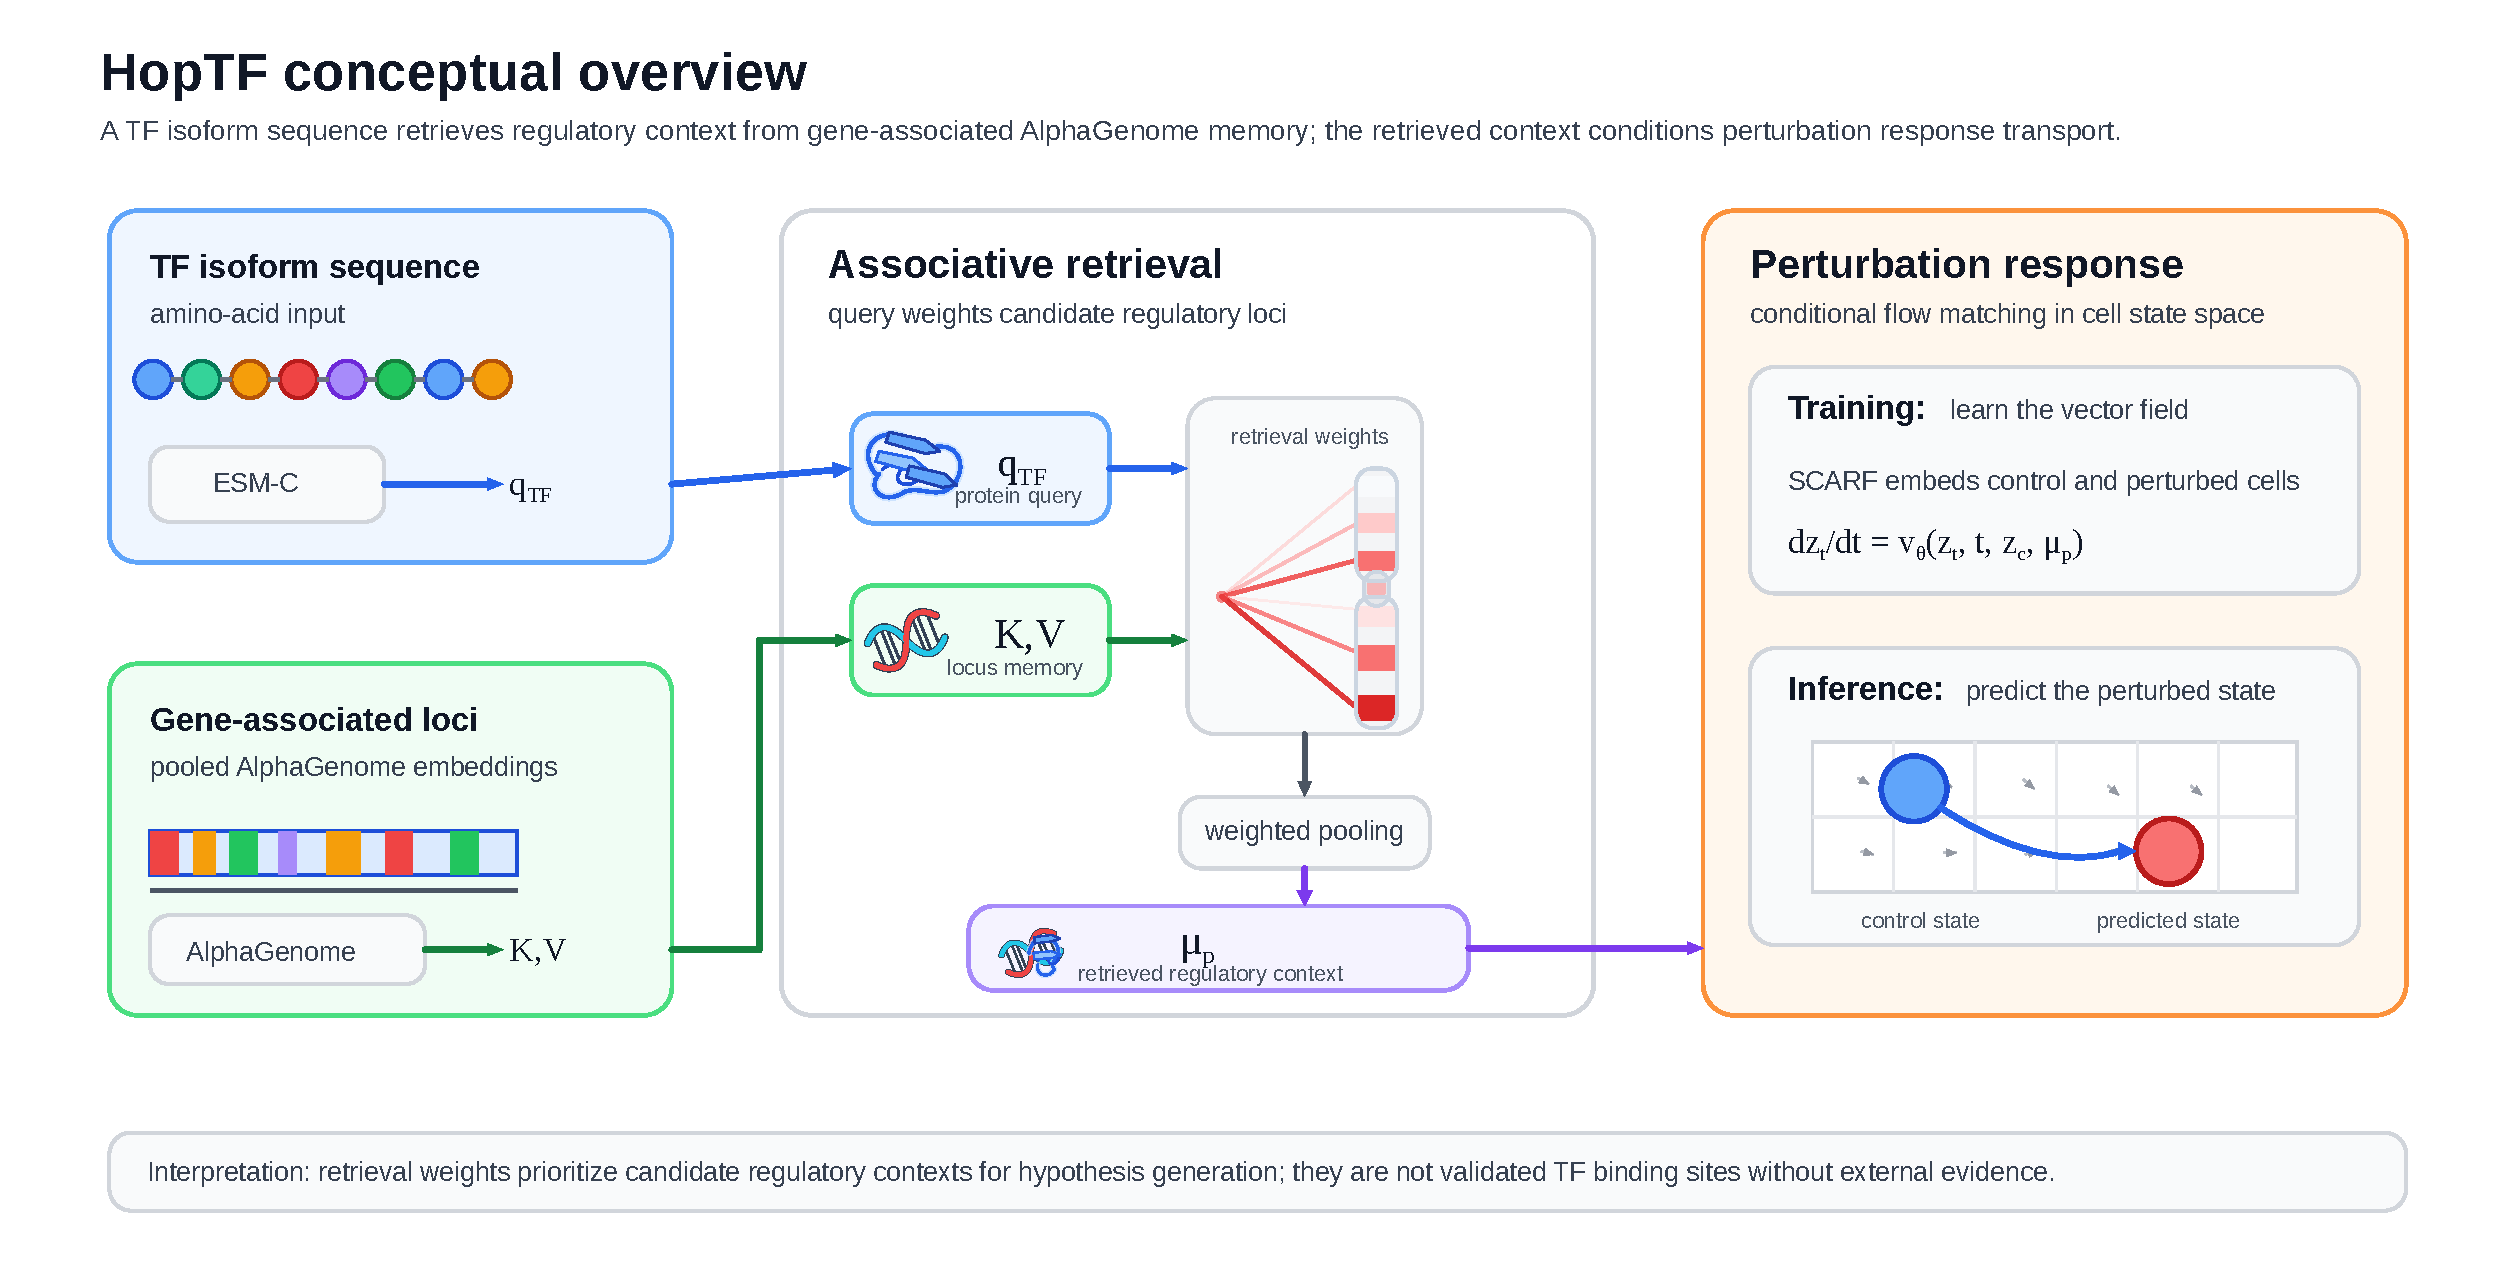
\includegraphics[width=\linewidth]{figures/hoptf_model_overview.pdf}
\caption{Overview of \hoptf. A TF isoform amino acid sequence is encoded into a protein query, gene-associated \ag\ embeddings provide a memory bank of locus keys and values, and associative retrieval produces a weighted regulatory context representation \(\mu_p\). This retrieved context conditions a flow model that predicts transport from unperturbed cells to cells after TF perturbation. Retrieval weights are interpreted as candidate hypotheses about regulatory context rather than validated binding sites.}
\label{fig:overview}
\end{figure}

\section{Positioning}

\hoptf\ is closest to three partially overlapping lines of work, but it is not identical to any of them. Single-cell perturbation models such as GEARS, CellOT, and scGPT focus on predicting transcriptional responses to genetic or chemical interventions \citep{roohani2023,bunne2023,cui2024}. These models are natural comparators for response prediction, but they usually represent the perturbation as a gene identity, graph feature, or learned embedding rather than as a TF protein sequence that explicitly queries candidate regulatory loci. Mechanistic regulatory network methods such as CellOracle and SCENIC+ provide richer biological structure through motifs, accessibility, enhancer-gene links, and regulatory networks \citep{kamimoto2023,gonzalezblas2023}. \hoptf\ is complementary to those methods: it does not replace motif or ChIP validation, but produces a learned retrieval distribution that can be audited against those sources.

Protein-aware TF-DNA binding models such as TransBind and TFBindFormer are closer in that they condition DNA sequence predictions on TF protein representations \citep{basnet2026,liutfbindformer2026}. Their endpoint, however, is local TF-DNA binding prediction on genomic sequence windows or ChIP-style labels. \hoptf\ instead retrieves from a genome-indexed regulatory memory and uses the retrieved state to condition aggregate response in cell state space. STRAND is a close transport model neighbor because it predicts single-cell perturbation responses using sequence-conditioned transport \citep{fu2026}. The direction of conditioning differs: STRAND conditions on regulatory DNA sequence at an intervention locus, whereas \hoptf\ uses TF protein sequence as the query into gene-associated regulatory memory.

This positioning determines the evaluation standard. A pure perturbation benchmark would ask only whether \hoptf\ beats covariates or generic baselines on held-out response prediction. A pure binding model would ask whether top-ranked loci match measured binding peaks. The goal here is narrower: test whether protein sequence can drive retrieval from regulatory memory in a way that is useful, sequence sensitive, and inspectable under weak aggregate supervision.

\section{Model and Evaluation}

\subsection{Sequence-conditioned regulatory memory}

Let \(x \in \mathbb{R}^G\) denote a single-cell expression vector, \(p\) a TF perturbation, and \(s_p\) the amino acid sequence of the perturbed TF isoform. Cells are embedded into a latent state \(z=E_{\mathrm{cell}}(x)\), and TF perturbation response is modeled in that latent space. Candidate regulatory contexts are represented by a memory bank of \(N=54{,}901\) gene-associated \ag\ entries. Each entry has a frozen 3072-dimensional pooled \ag\ embedding and metadata linking it to a gene-associated genomic context. The retrieval model consumes these pooled embeddings directly; it does not construct a new sliding-window genome tiling. For motif and ReMap diagnostics only, entries are mapped to 1~kb TSS-centered validation windows.

The memory uses learned task-specific projections on top of frozen foundation features:
\begin{align}
    k_i &= W_K h_i^{\mathrm{AG}}, &
    v_i &= W_V h_i^{\mathrm{AG}}, &
    q_p &= W_Q E_{\mathrm{prot}}(s_p).
\end{align}
Here \(k_i\) is a locus key, \(v_i\) is a retrieved value, and \(q_p\) is the TF protein query. The unmasked retrieval distribution and pooled regulatory context representation are
\begin{align}
    \alpha_{pi} &= \frac{\exp(\beta q_p^\top k_i)}{\sum_{j=1}^N \exp(\beta q_p^\top k_j)}, &
    \mu_p &= \sum_{i=1}^N \alpha_{pi}v_i.
\end{align}
The inverse temperature \(\beta\) controls retrieval concentration. Low \(\beta\) yields diffuse averaging across many loci; high \(\beta\) concentrates mass on fewer entries. The reported retrieval analyses use the shared unmasked memory derived from \ag. Accessibility priors by cluster or hard locus masks are left for future work because the current staged cell representation is derived from RNA and is not a calibrated accessibility predictor.

The implemented feature stack is intentionally lightweight. \esm\ is used as a frozen 600M-parameter protein encoder with mean pooling over non-special tokens, producing a 1152-dimensional isoform embedding \citep{evolutionaryscale2024}. The \ag\ memory is loaded from a fixed gene-pooled archive and is not fine-tuned. \scarf\ is also frozen and is used only as a cell state and response representation. The trainable pieces are task-specific projections and endpoint predictors built on top of these frozen features. This design keeps the retrieval distribution interpretable: when a TF sequence changes, the observed response and retrieval changes can be attributed to the sequence-derived query and fixed memory rather than to broad fine-tuning of the underlying foundation models.

The retrieval module is differentiable, but the supervision is weak. The model is not given labels for which locus mediates a TF response. Instead, gradients from response prediction shape the protein query projection and endpoint predictor, while the locus activation distribution remains a latent intermediate. This is the multiple-instance structure of the problem: the candidate loci form the bag, the TF sequence is the query over the bag, and the observed response after perturbation is the bag-level target. Because labels at the locus level are absent, retrieval weights must be interpreted as hypotheses rather than as binding probabilities.

\subsection{Conditional response objective}

The intended endpoint model is a conditional vector field in cell state latent space. For a control cell latent \(z_0\), a perturbed cell latent \(z_1\), and a retrieved regulatory context vector \(\mu_{0p}\), \hoptf\ represents perturbation response as
\begin{equation}
    \frac{d z_t}{dt} = v_\theta(z_t, t, z_0, \mu_{0p}), \qquad t \in [0,1].
\end{equation}
This makes the retrieval vector part of the transport condition rather than a separate post hoc explanation. In the flow-matching formulation, minibatch optimal transport couplings pair control and perturbed latents for the same TF perturbation \citep{tong2024cfm,tong2024sf2m}. For \(t \sim \mathrm{Uniform}(0,1)\), define
\begin{align}
    z_t &= (1-t)z_0 + t z_1, &
    u_t &= z_1-z_0.
\end{align}
The conditional flow-matching loss is
\begin{equation}
    \mathcal{L}_{\mathrm{CFM}} =
    \mathbb{E}_{p,(z_0,z_1),t}\left[
    \left\|v_\theta(z_t,t,z_0,\mu_{0p}) - u_t\right\|_2^2
    \right].
\end{equation}
The flow objective is the reason the retrieved representation is coupled to response prediction: the model is rewarded only if the retrieved context helps explain the direction from control to perturbed cells. In this submission, the strongest reported endpoint analyses use frozen \scarf\ response vectors rather than decoded expression trajectories. We therefore report held-out \scarf\ response prediction, variant-induced response changes, and retrieval diagnostics, and we treat the earlier PCA endpoint transport runs as sensitivity evidence.

The current retrieval logits are intentionally simple:
\begin{equation}
    r_{pi}=\beta q_p^\top k_i.
\end{equation}
This is the unmasked shared memory setting. A richer model aware of cell state could add a cluster or accessibility term,
\begin{equation}
    r_{cpi}=\beta q_p^\top k_i + \lambda A_{ci},
\end{equation}
where \(A_{ci}\) is an availability prior for locus \(i\) in cell state cluster \(c\). We do not activate this term in the reported experiments, because the staged endpoint is RNA-derived and not a calibrated accessibility measurement. This design choice keeps the current claims narrower: retrieval is sequence-conditioned and genome-indexed, but not yet masked by cell type accessibility.

\subsection{Response endpoint and controls}

The primary response endpoint is frozen \scarf\ latent response space \citep{scarf2025}. For each perturbation, the observed response vector is the mean \scarf\ latent of cells after TF perturbation minus the mean \scarf\ latent of control cells. The local staged TF Atlas subset contains 671,453 cells, 3,266 perturbation labels, 2,000 control cells, and 512-dimensional \scarf\ latents. Primary prediction uses five-fold grouped held-out-gene splits, so isoforms and sequence-derived rows from the same TF gene do not leak across folds.

The central predictive question is whether sequence features improve held-out response prediction in \scarf\ space after measured non-sequence covariates are included. We therefore compare sequence feature sets against protein length, ORF length, and recovered cell count. Variant analyses use matched within-isoform comparisons: pathogenic missense variants are compared against matched random substitutions and evidence-tiered benign/control substitutions. Retrieval diagnostics use entropy, effective number of loci, top-\(k\) mass, variant-induced retrieval movement, and motif/ReMap support. We do not report decoded gene expression recovery or target prediction at gene level.

These controls are important because TF Atlas response metrics are not independent of library and recovery structure. Protein length and ORF length affect packaging and overexpression, while recovered cell count can reflect both technical recovery and biological response strength. A model using sequence is therefore not convincing unless it is compared against those measured quantities. The primary \scarf\ benchmark uses mean squared error between predicted and observed response vectors, with cosine similarity as a secondary geometry diagnostic. Matched context heatmaps report percent MSE change relative to the length/ORF/cell-count baseline, so negative values would indicate that adding sequence information improves prediction.

\subsection{Comparison design}

The evaluation is organized around two separate questions. First, does information from sequence improve held-out TF response prediction beyond simple measured quantities? Second, even if the response benchmark is negative, does the retrieval mechanism behave like a sequence-sensitive regulatory memory layer? Table~\ref{tab:main_comparison_design} summarizes the design and separates completed analyses from planned but unreported ablations.

\begin{table*}[t]
\centering
\caption{Main comparison design. The reported paper emphasizes completed comparisons and explicitly labels uncompleted ablations as future work rather than results.}
\label{tab:main_comparison_design}
\resizebox{\textwidth}{!}{%
\begin{tabular}{p{0.22\textwidth}p{0.39\textwidth}p{0.25\textwidth}p{0.10\textwidth}}
\toprule
\textbf{Comparison} & \textbf{Description} & \textbf{Question tested} & \textbf{Status} \\
\midrule
Length / ORF / cell-count inputs & Predict \scarf\ response from protein length, ORF length, and recovered perturbation cell count. & How much of the endpoint is explained by measured non-sequence quantities? & Completed \\
Raw and projected \esm & Compare frozen \esm\ features directly and after projection into \ag\ key space. & Do protein sequence features improve response prediction beyond the covariate baseline? & Completed \\
Raw and projected \esmdbp & Repeat the sequence feature benchmark using a DBP-specialized ESM2-style encoder. & Does a protein encoder specialized for DNA binding outperform general \esm? & Completed \\
Shuffled sequence features & Mismatch or shuffle sequence features in the controlled benchmark. & Are apparent sequence effects stronger than a negative control sequence feature? & Completed where available \\
Matched variant substitutions & Compare pathogenic missense variants against matched random and benign/control substitutions. & Do amino acid changes perturb predicted response and retrieval more than controls? & Completed \\
\(\beta\) sweep & Vary the retrieval inverse temperature while holding the memory and query construction fixed. & Does the retrieval layer move from diffuse to concentrated associative lookup as intended? & Completed \\
Motif/ReMap support & Test whether top retrieved 1~kb validation windows overlap same-symbol JASPAR motifs or ReMap peaks. & Are loci with high retrieval weight independently supported as binding-related candidates? & Completed, weak support \\
TF-ID embedding baseline & Replace protein sequence with a learned identity embedding. & Is protein sequence better than memorizing TF identity? & Future work \\
Random memory ablation & Replace \ag\ memory with random or shuffled locus embeddings in the primary endpoint model. & Does the memory derived from genome features itself add signal beyond an addressable parameter set? & Future work \\
Cell state accessibility mask & Add cluster-level priors or availability priors specific to cell state over loci. & Does retrieval with cell context improve biological specificity? & Future work \\
\bottomrule
\end{tabular}%
}
\end{table*}

The implemented response prediction comparisons are deliberately conservative. All primary \scarf\ metrics use held-out TF genes rather than random held-out cells, because random cell splits would allow isoforms from the same TF gene to appear in both training and test folds. Perturbation metadata are joined by perturbation identifier and include recovered cell count, protein length, ORF length, gene symbol, isoform identifier, and isoform embedding identifier. The benchmark excludes rows with insufficient recovered cells in shared modeling scripts, pools GFP and mCherry controls to form the control reference mean, and evaluates the latent response vector directly. We do not decode \scarf\ predictions back to expression, and we do not report target recovery at gene level.

Retrieval is evaluated separately from response prediction. The diagnostic metrics include entropy \(H(\alpha)\), effective number of retrieved loci, top-\(k\) mass, top-\(k\) overlap across \(\beta\), variant-induced movement of the retrieval distribution, and motif or ReMap support among validation windows associated with entries with high retrieval weight. This separation is important because a response model can fail to improve MSE while the retrieval layer still behaves as a useful probe of sequence sensitivity. Conversely, a predictive response model would not by itself validate the retrieved loci as regulatory mechanisms.

\subsection{Variant control construction}

The matched benign/control panel is constructed as a control set tiered by evidence for local HopTF isoforms, not as a claim that every retained substitution is biologically neutral. Natural human evidence is used first. ClinVar benign or likely benign variants, gnomAD missense variants with population tolerance evidence, and MaveDB assay rows with high function scores are accepted only after exact protein coordinate checking against the local HopTF isoform sequence \citep{landrum2025clinvar,karczewski2020gnomad,esposito2019mavedb}. The reference amino acid at the one-based position must match the local wild-type sequence, and mutant proteins are regenerated from the local sequence rather than copied from source records. Ambiguous coordinate mappings, non-missense changes, conflicting labels, and pathogenic or likely pathogenic annotations are excluded from the control set.

Because many TF isoforms have few natural benign/control variants, the fixed size panel uses synthetic controls supported by ortholog evidence before falling back to deterministic conservative substitutions. For a control supported by ortholog evidence, the alternate residue must be observed at the aligned position in an Ensembl Compara ortholog \citep{dyer2025ensembl}. The ortholog and local proteins are aligned, the local reference residue must match the proposed position, and the candidate must pass conservative chemistry filters and sensitive position filters. In the final construction, Pfam domain architecture agreement is also required before accepting a substitution supported by ortholog evidence \citep{mistry2021pfam}. Table~\ref{tab:main_variant_control_tiers} reports the tier composition used in the capped variant control table.

\begin{table*}[t]
\centering
\caption{Evidence tiers for benign/control variant construction. Tier 5 rows are retained only to preserve a fixed design of 10 control substitutions and are not treated as independent benign evidence.}
\label{tab:main_variant_control_tiers}
\small
\begin{tabular}{@{}>{\raggedright\arraybackslash}p{0.12\textwidth}>{\raggedright\arraybackslash}p{0.55\textwidth}>{\centering\arraybackslash}p{0.11\textwidth}>{\centering\arraybackslash}p{0.11\textwidth}@{}}
\toprule
\textbf{Tier} & \textbf{Inclusion rule} & \textbf{Uncapped rows} & \textbf{Selected rows} \\
\midrule
Tier 1 & Clinical benign/control: ClinVar benign, likely benign, or benign/likely benign; no conflicts; exact local isoform match & 2,064 & 1,817 \\
Tier 2a & Strong population-tolerated: gnomAD v4.1 exome missense row; no disease/conflict annotation; exact local isoform match; group-maximum AF at least 1\% & 2,734 & 2,065 \\
Tier 2b & Moderate population-tolerated: gnomAD v4.1 exome missense row passing staged population-tolerance filters but below strong threshold & 4,789 & 1,940 \\
Tier 3 & Functional-assay control: MaveDB high-score assay row; exact local isoform match; unambiguous high-score-as-more-functional convention; no local ClinVar deleterious match & 132 & 67 \\
Tier 4 & Ortholog-supported synthetic control: alternate residue is observed at the aligned position in an Ensembl Compara ortholog; chemistry, sensitive position, and Pfam architecture filters pass & -- & 18,600 \\
Tier 5 & Legacy conservative fallback control: deterministic conservative substitution used only when Tiers 1--4 do not provide enough rows for exactly 10 controls per isoform & -- & 8,151 \\
\bottomrule
\end{tabular}
\end{table*}

The natural evidence table contains 9,719 rows across 717 isoforms; 435 isoforms have at least 10 natural rows. The capped table contains 32,640 rows: 5,889 natural evidence rows, 18,600 ortholog-supported tier 4 rows, and 8,151 tier 5 fallback rows. A total of 2,259 isoforms need no tier 5 fallback. These counts matter for interpretation. When pathogenic variants are compared against the benign/control panel, the strongest claim is that pathogenic substitutions produce larger absolute predicted response changes than this matched control mixture. The tiered design does not prove that every control substitution is functionally silent, and tier 5 should be excluded or reported separately in future tolerance-aware training.

\begin{figure}[t]
\centering
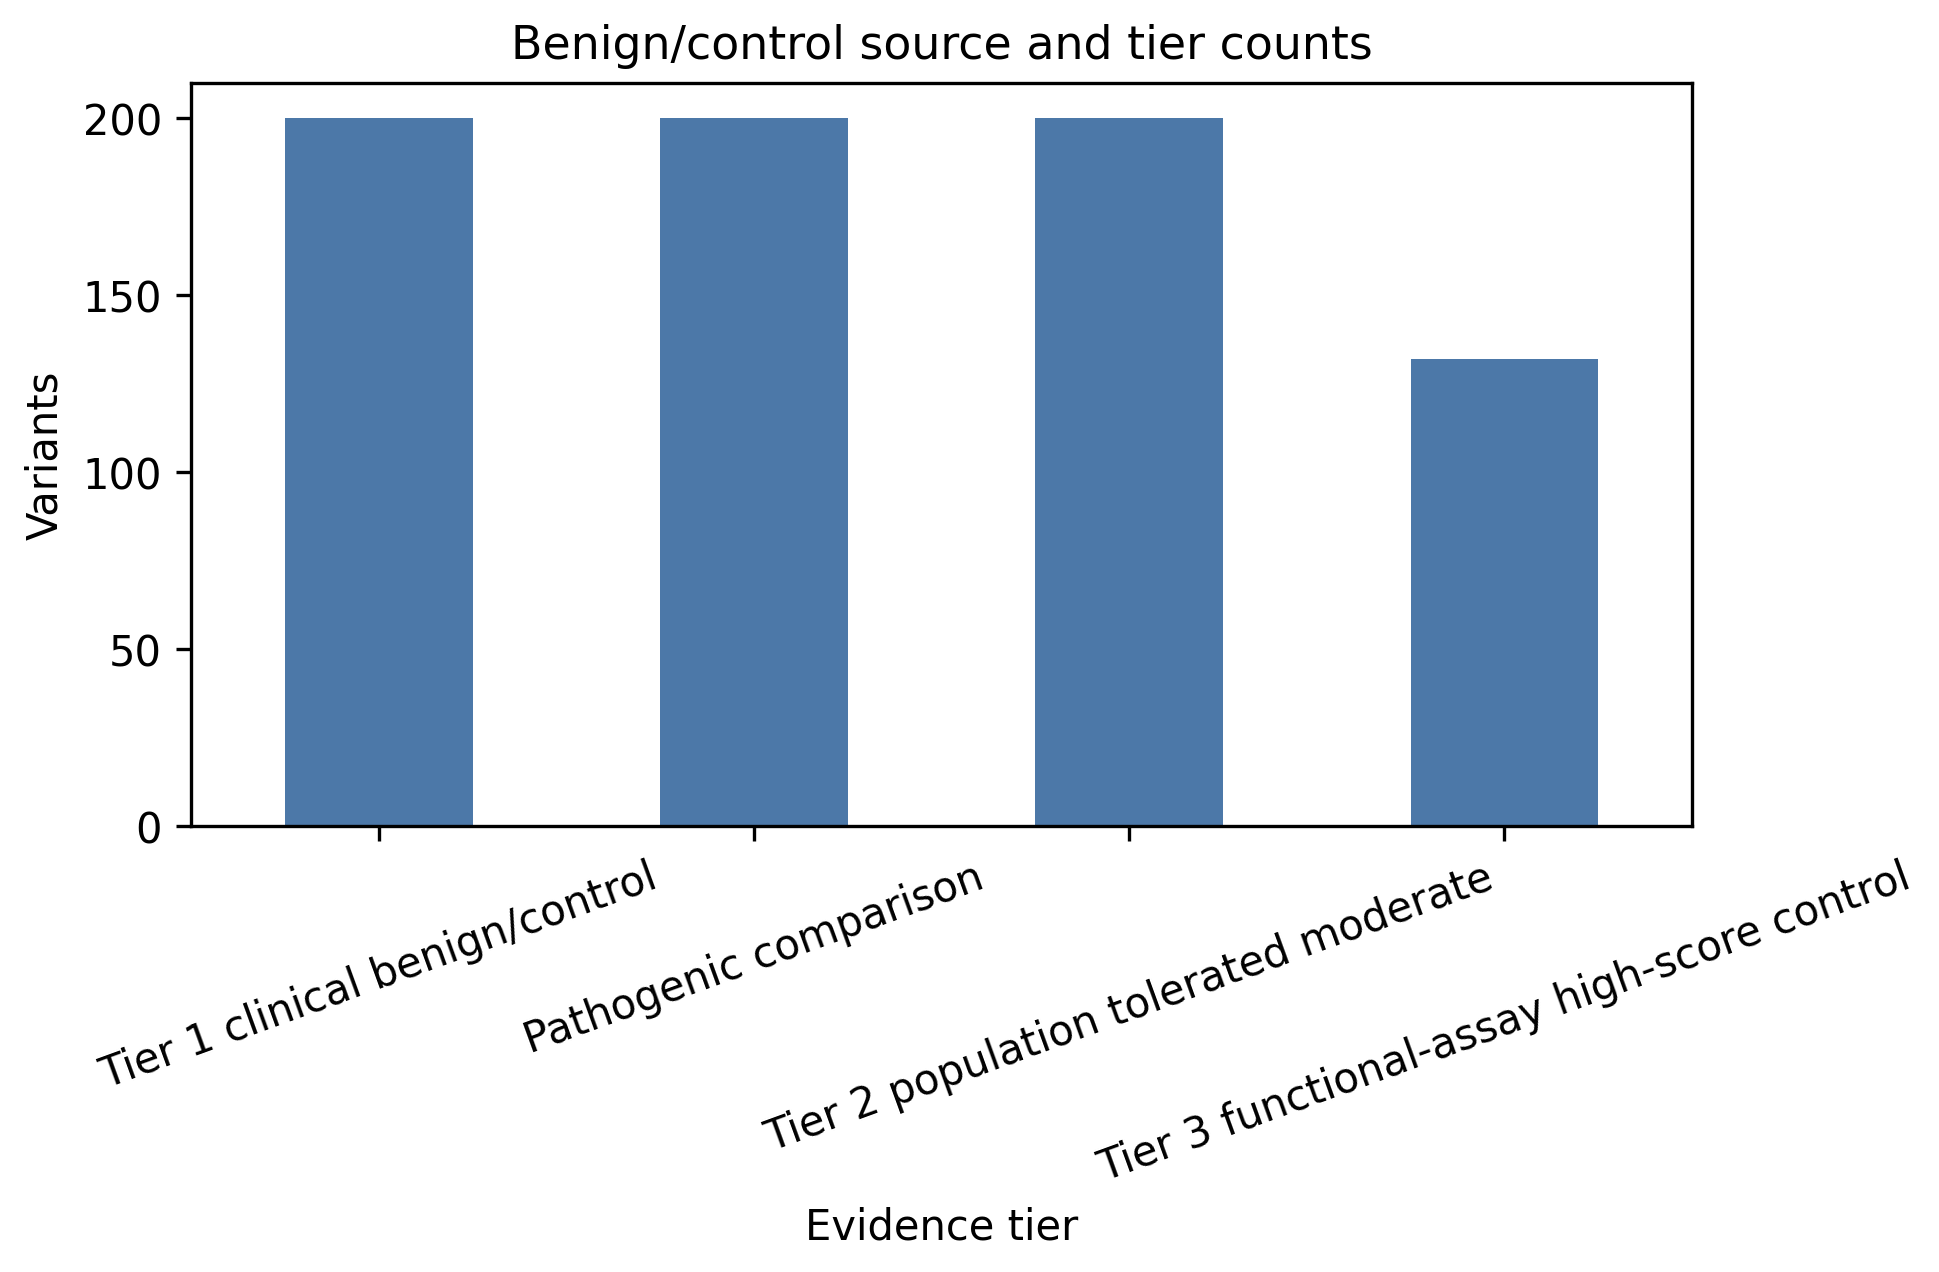
\includegraphics[width=0.76\linewidth]{figures/benign_control_tier_counts.png}
\caption{Composition of the benign/control variant panel tiered by evidence. Natural clinical, population, and functional assay evidence is prioritized first; tolerated substitutions supported by ortholog evidence fill many remaining fixed size slots; fallback controls are retained only where needed for exactly 10 variants per TF isoform.}
\label{fig:main_benign_control_tier_counts}
\end{figure}

\section{Results}

\subsection{SCARF benchmark limits the predictive claim}

In the primary \scarf\ benchmark, the covariate-only model using protein length, ORF length, and recovered cell count had the lowest held-out-gene MSE among the tested feature sets. Projected \esm\ was the strongest sequence feature set, but it did not improve over those measured covariates in the all-held-out-gene comparison or in matched protein-length, recovered-cell-count, and joint matched contexts. Lower MSE is better in Table~\ref{tab:scarf_sequence_benchmark}, and negative percent change would indicate improvement in Figure~\ref{fig:scarf_sequence_improvement_heatmap}.

\begin{table}[t]
\centering
\caption{Controlled \scarf\ sequence benchmark. Lower MSE is better. Percent change is relative to the model using protein length, ORF length, and recovered cell count.}
\label{tab:scarf_sequence_benchmark}
\resizebox{\linewidth}{!}{%
\begin{tabular}{lccc}
\toprule
\textbf{Feature set} & \textbf{MSE} & \textbf{MSE change} & \textbf{Mean cosine} \\
\midrule
Length + ORF + cell count & \(8.18\times 10^{-8}\) & 0.0\% & 0.8402 \\
Length + ORF + cell count + projected \esm & \(8.42\times 10^{-8}\) & +2.9\% & 0.8317 \\
Length + ORF + cell count + raw \esm & \(8.72\times 10^{-8}\) & +6.5\% & 0.8291 \\
Projected \esm\ only & \(8.74\times 10^{-8}\) & +6.8\% & 0.8326 \\
Raw \esm\ only & \(9.11\times 10^{-8}\) & +11.3\% & 0.8299 \\
Shuffled \esm\ after covariates & \(9.42\times 10^{-8}\) & +15.2\% & 0.8290 \\
Training-set mean response & \(3.65\times 10^{-7}\) & +346.0\% & 0.0000 \\
\bottomrule
\end{tabular}%
}
\end{table}

\begin{figure}[t]
\centering
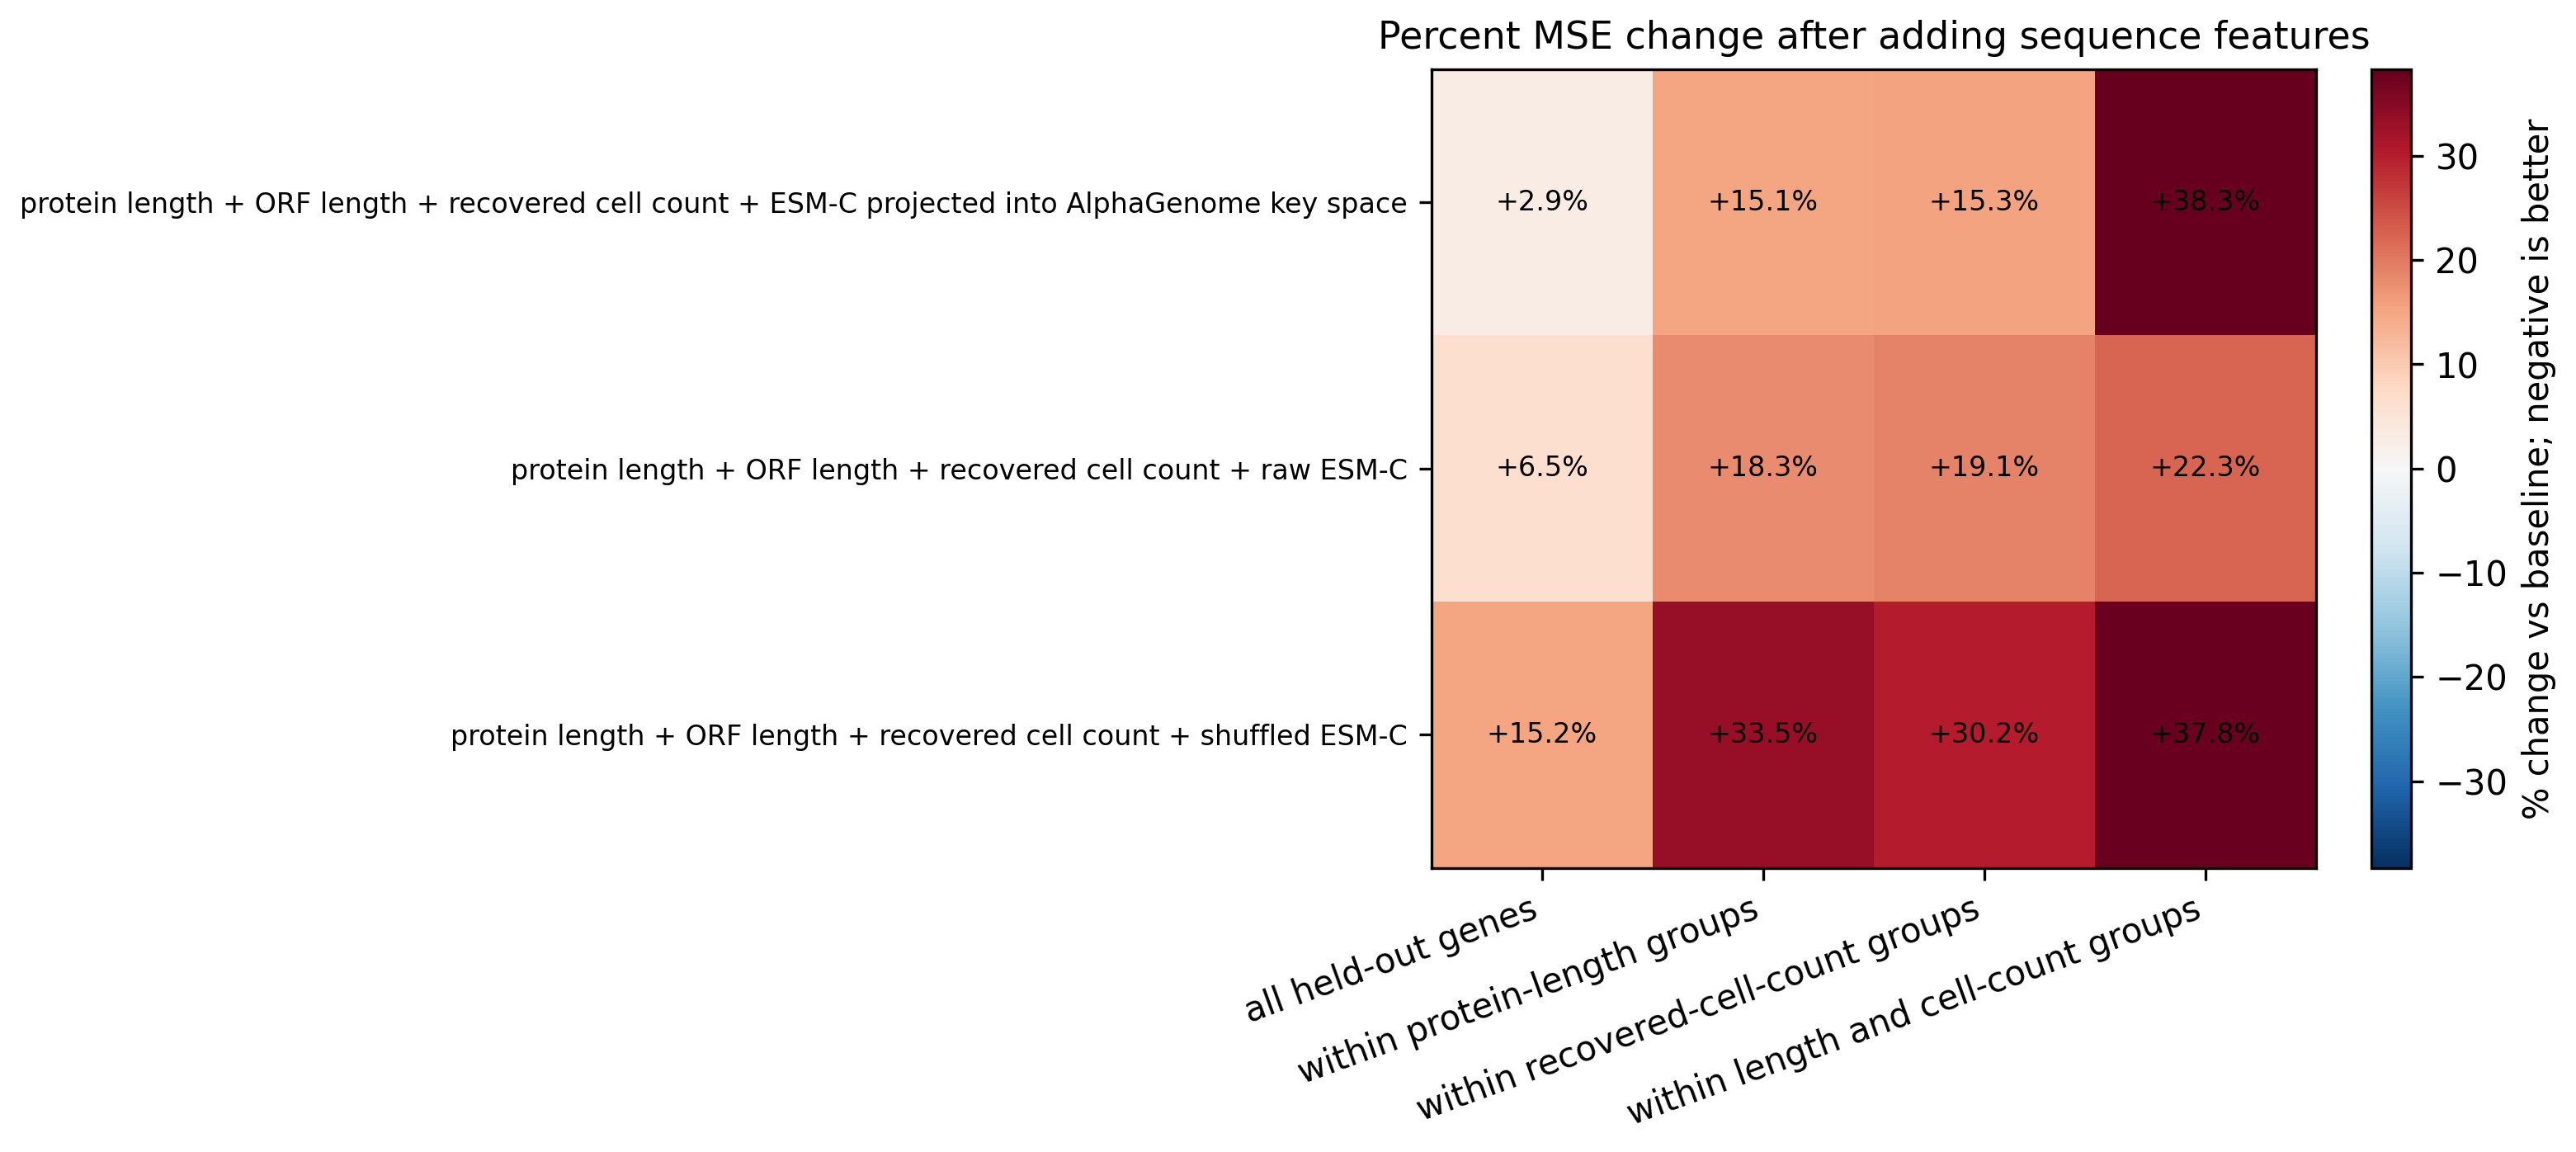
\includegraphics[width=0.88\linewidth]{figures/scarf_sequence_improvement_heatmap.png}
\caption{Matched context \scarf\ sequence benchmark. Values are percent MSE changes relative to the covariate-only baseline; negative values would indicate improvement. Projected \esm\ is better than raw or shuffled \esm, but adding sequence features does not improve over measured covariates.}
\label{fig:scarf_sequence_improvement_heatmap}
\end{figure}

This is a negative result for the broad predictive claim. The older PCA benchmark remains useful as a sensitivity analysis (Appendix~\ref{app:pca_sensitivity}), and the \scarf\ benchmark still shows that projected \esm\ is the best sequence feature set tested. However, the current results do not support claiming that features derived from sequence improve general held-out TF response prediction once measured covariates are included. The rest of the paper therefore focuses on sequence sensitivity and retrieval diagnostics rather than broad predictive superiority.

\begin{figure}[t]
\centering
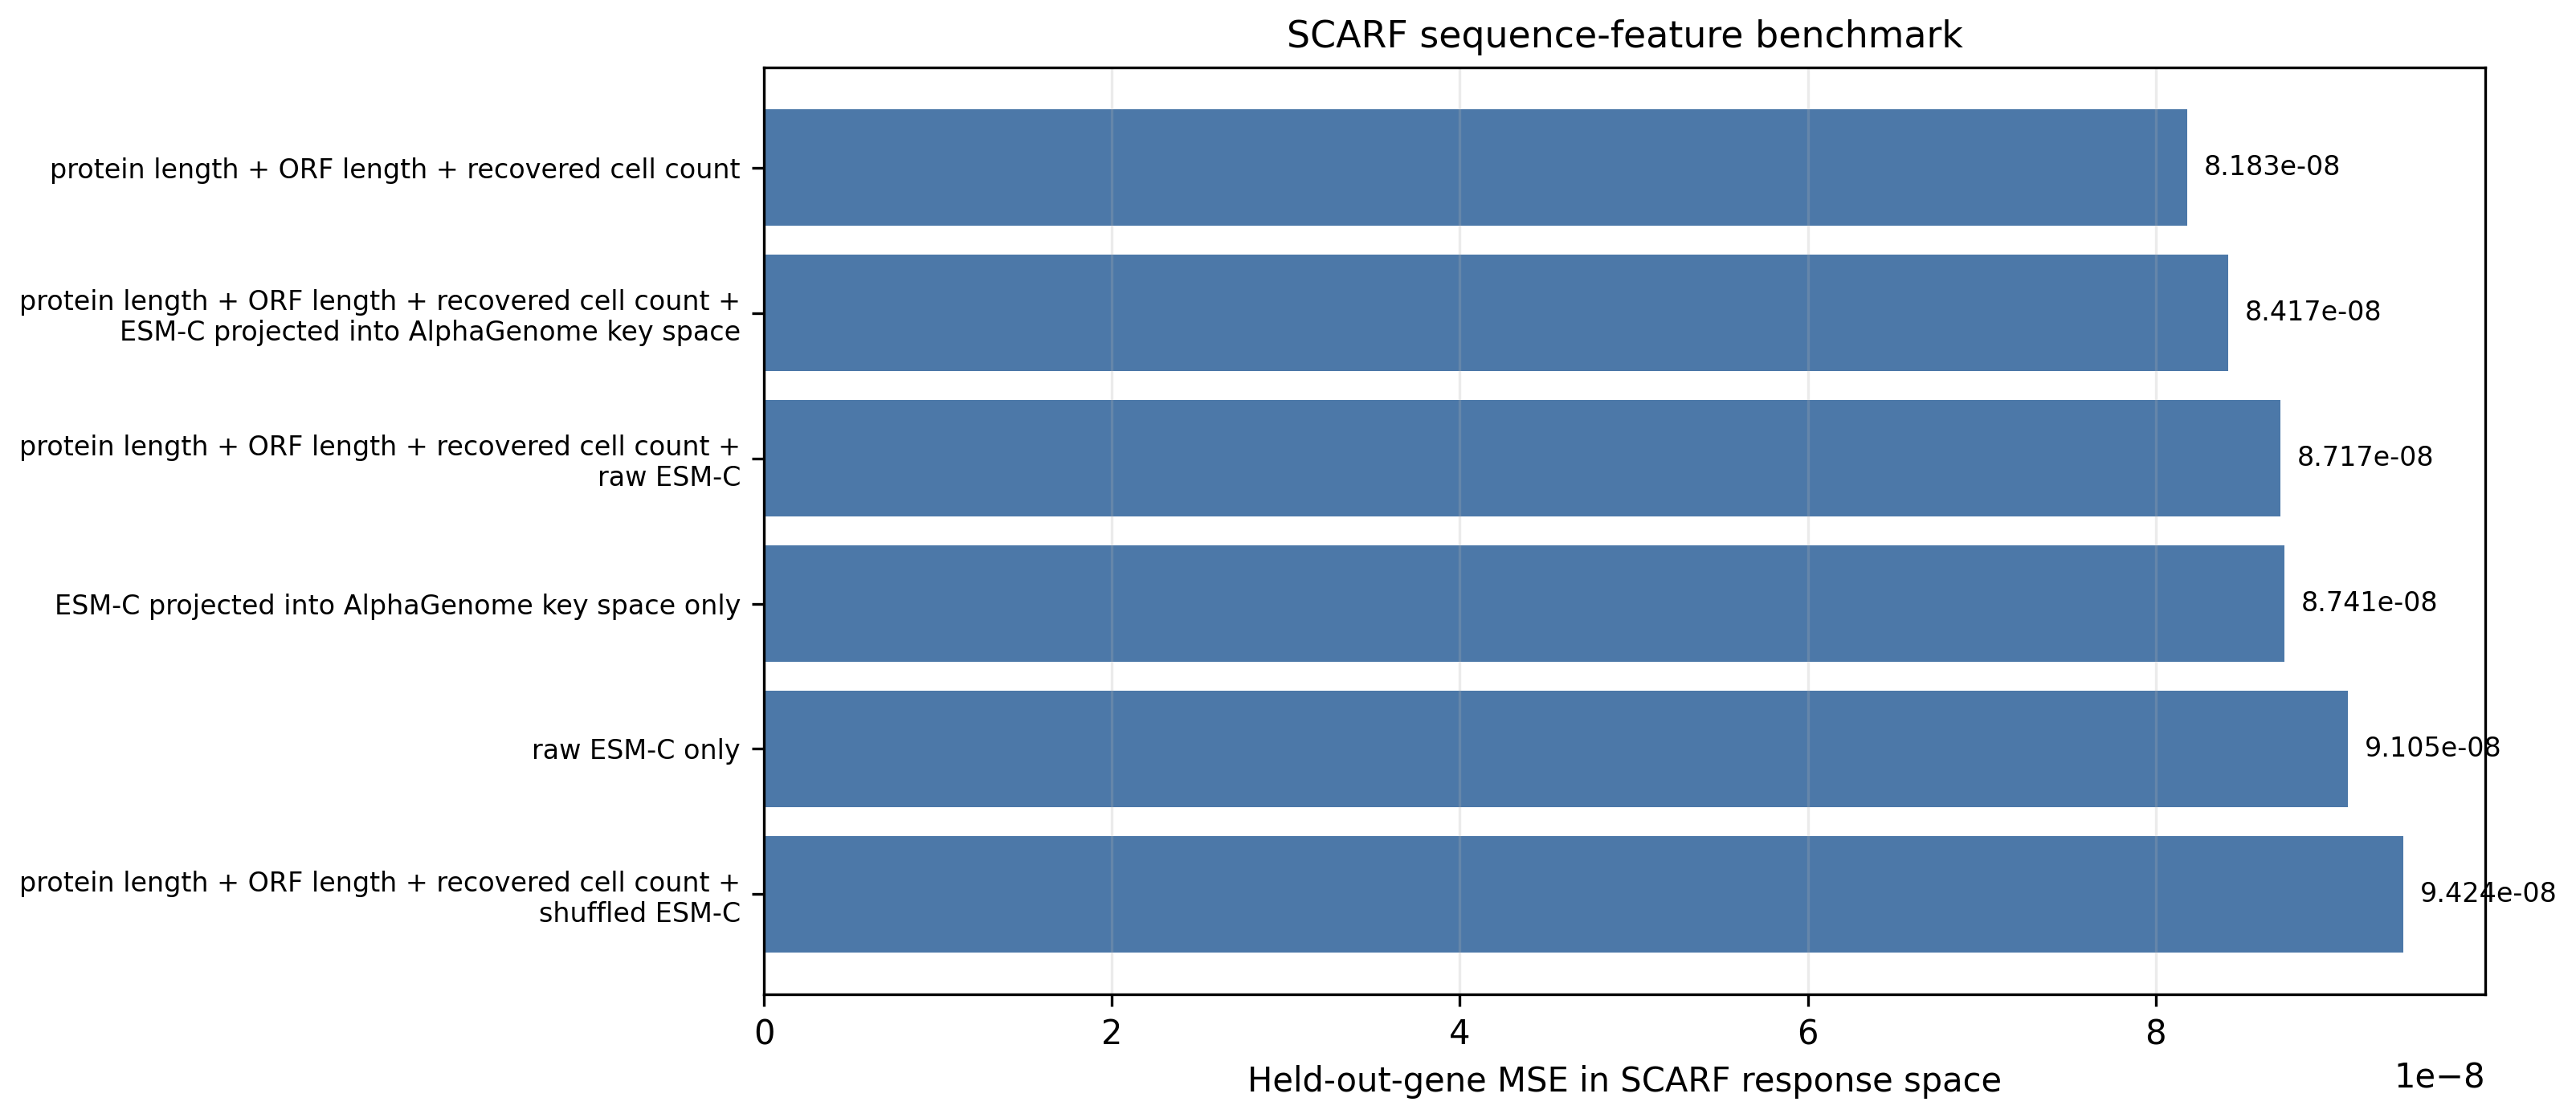
\includegraphics[width=0.86\linewidth]{figures/scarf_sequence_feature_benchmark.png}
\caption{Controlled \scarf\ sequence feature benchmark. Lower MSE is better. Protein length, ORF length, and recovered cell count are difficult to beat; projected \esm\ plus these covariates is the strongest model using sequence but does not improve over the covariate-only baseline in this response representation.}
\label{fig:scarf_sequence_feature_benchmark}
\end{figure}

\subsection{PCA sensitivity suggests modest sequence signal}

Before switching the primary endpoint to frozen \scarf\ response space, we evaluated a PCA latent response representation. This older benchmark is not the main claim because the PCA endpoint is less aligned with the final response representation and is more sensitive to preprocessing choices. It is nevertheless useful as a sensitivity check: it asks whether the negative \scarf\ result is the only observed pattern or whether sequence features sometimes help under a different endpoint.

\begin{table}[t]
\centering
\caption{Older PCA latent sensitivity benchmark. Lower MSE is better. This result is retained as secondary evidence, not as the primary response prediction claim.}
\label{tab:main_pca_sensitivity}
\resizebox{\linewidth}{!}{%
\begin{tabular}{lccc}
\toprule
\textbf{Feature set} & \textbf{MSE} & \textbf{MSE change} & \textbf{Mean cosine} \\
\midrule
Length + ORF + cell count & 6.5996 & 0.0\% & 0.3970 \\
Length + ORF + cell count + projected \esm & 6.2879 & -4.7\% & 0.4548 \\
Length + ORF + cell count + raw \esm & 6.8774 & +4.2\% & 0.3861 \\
Projected \esm\ only & 6.8806 & +4.3\% & 0.3395 \\
Raw \esm\ only & 7.3078 & +10.7\% & 0.3024 \\
Shuffled \esm\ after covariates & 7.5761 & +14.8\% & 0.1679 \\
Training-set mean perturbed state & 37.6192 & +470.0\% & -0.4740 \\
\bottomrule
\end{tabular}%
}
\end{table}

The PCA latent result is consistent with a modest sequence signal after covariates: projected \esm\ plus length, ORF length, and recovered cell count lowered MSE by 4.7\% relative to covariates alone. The same pattern did not survive as a main predictive win in \scarf\ space, so we do not present it as evidence that \hoptf\ improves general response prediction. Instead, it supports a narrower interpretation: the sequence representation is not arbitrary noise, projected \esm\ is more useful than raw or shuffled sequence features in at least one response representation, and endpoint choice materially affects the strength of the predictive claim.

\subsection{Missense variants perturb response and retrieval}

We next used TF missense variants as a diagnostic for sequence sensitivity. This analysis does not ask whether \hoptf\ classifies clinical variants. Instead, it asks whether changing a TF amino acid sequence moves the predicted perturbation response more than matched control substitutions. Because damaging TF variants may weaken, strengthen, or redirect response, the primary metric is absolute WT-vs-mutant response change rather than signed weakening.

\begin{table}[t]
\centering
\caption{\scarf\ matched variant validation. Positive paired differences mean pathogenic variants changed predicted perturbed cell state activity more than the matched control group.}
\label{tab:matched_variant_validation}
\resizebox{\linewidth}{!}{%
\begin{tabular}{lcccc}
\toprule
\textbf{Comparison} & \textbf{Metric} & \textbf{Sets} & \textbf{Median diff.} & \textbf{Wilcoxon \(p\)} \\
\midrule
Pathogenic vs. matched random & Signed weakening & 189 & 0.0138 & 0.9735 \\
Pathogenic vs. matched random & Absolute disruption & 189 & 0.0111 & 0.0084 \\
Pathogenic vs. benign/control & Signed weakening & 158 & 0.0451 & 0.9996 \\
Pathogenic vs. benign/control & Absolute disruption & 158 & 0.0346 & \(5.46\times 10^{-6}\) \\
\bottomrule
\end{tabular}%
}
\end{table}

\begin{figure}[t]
\centering
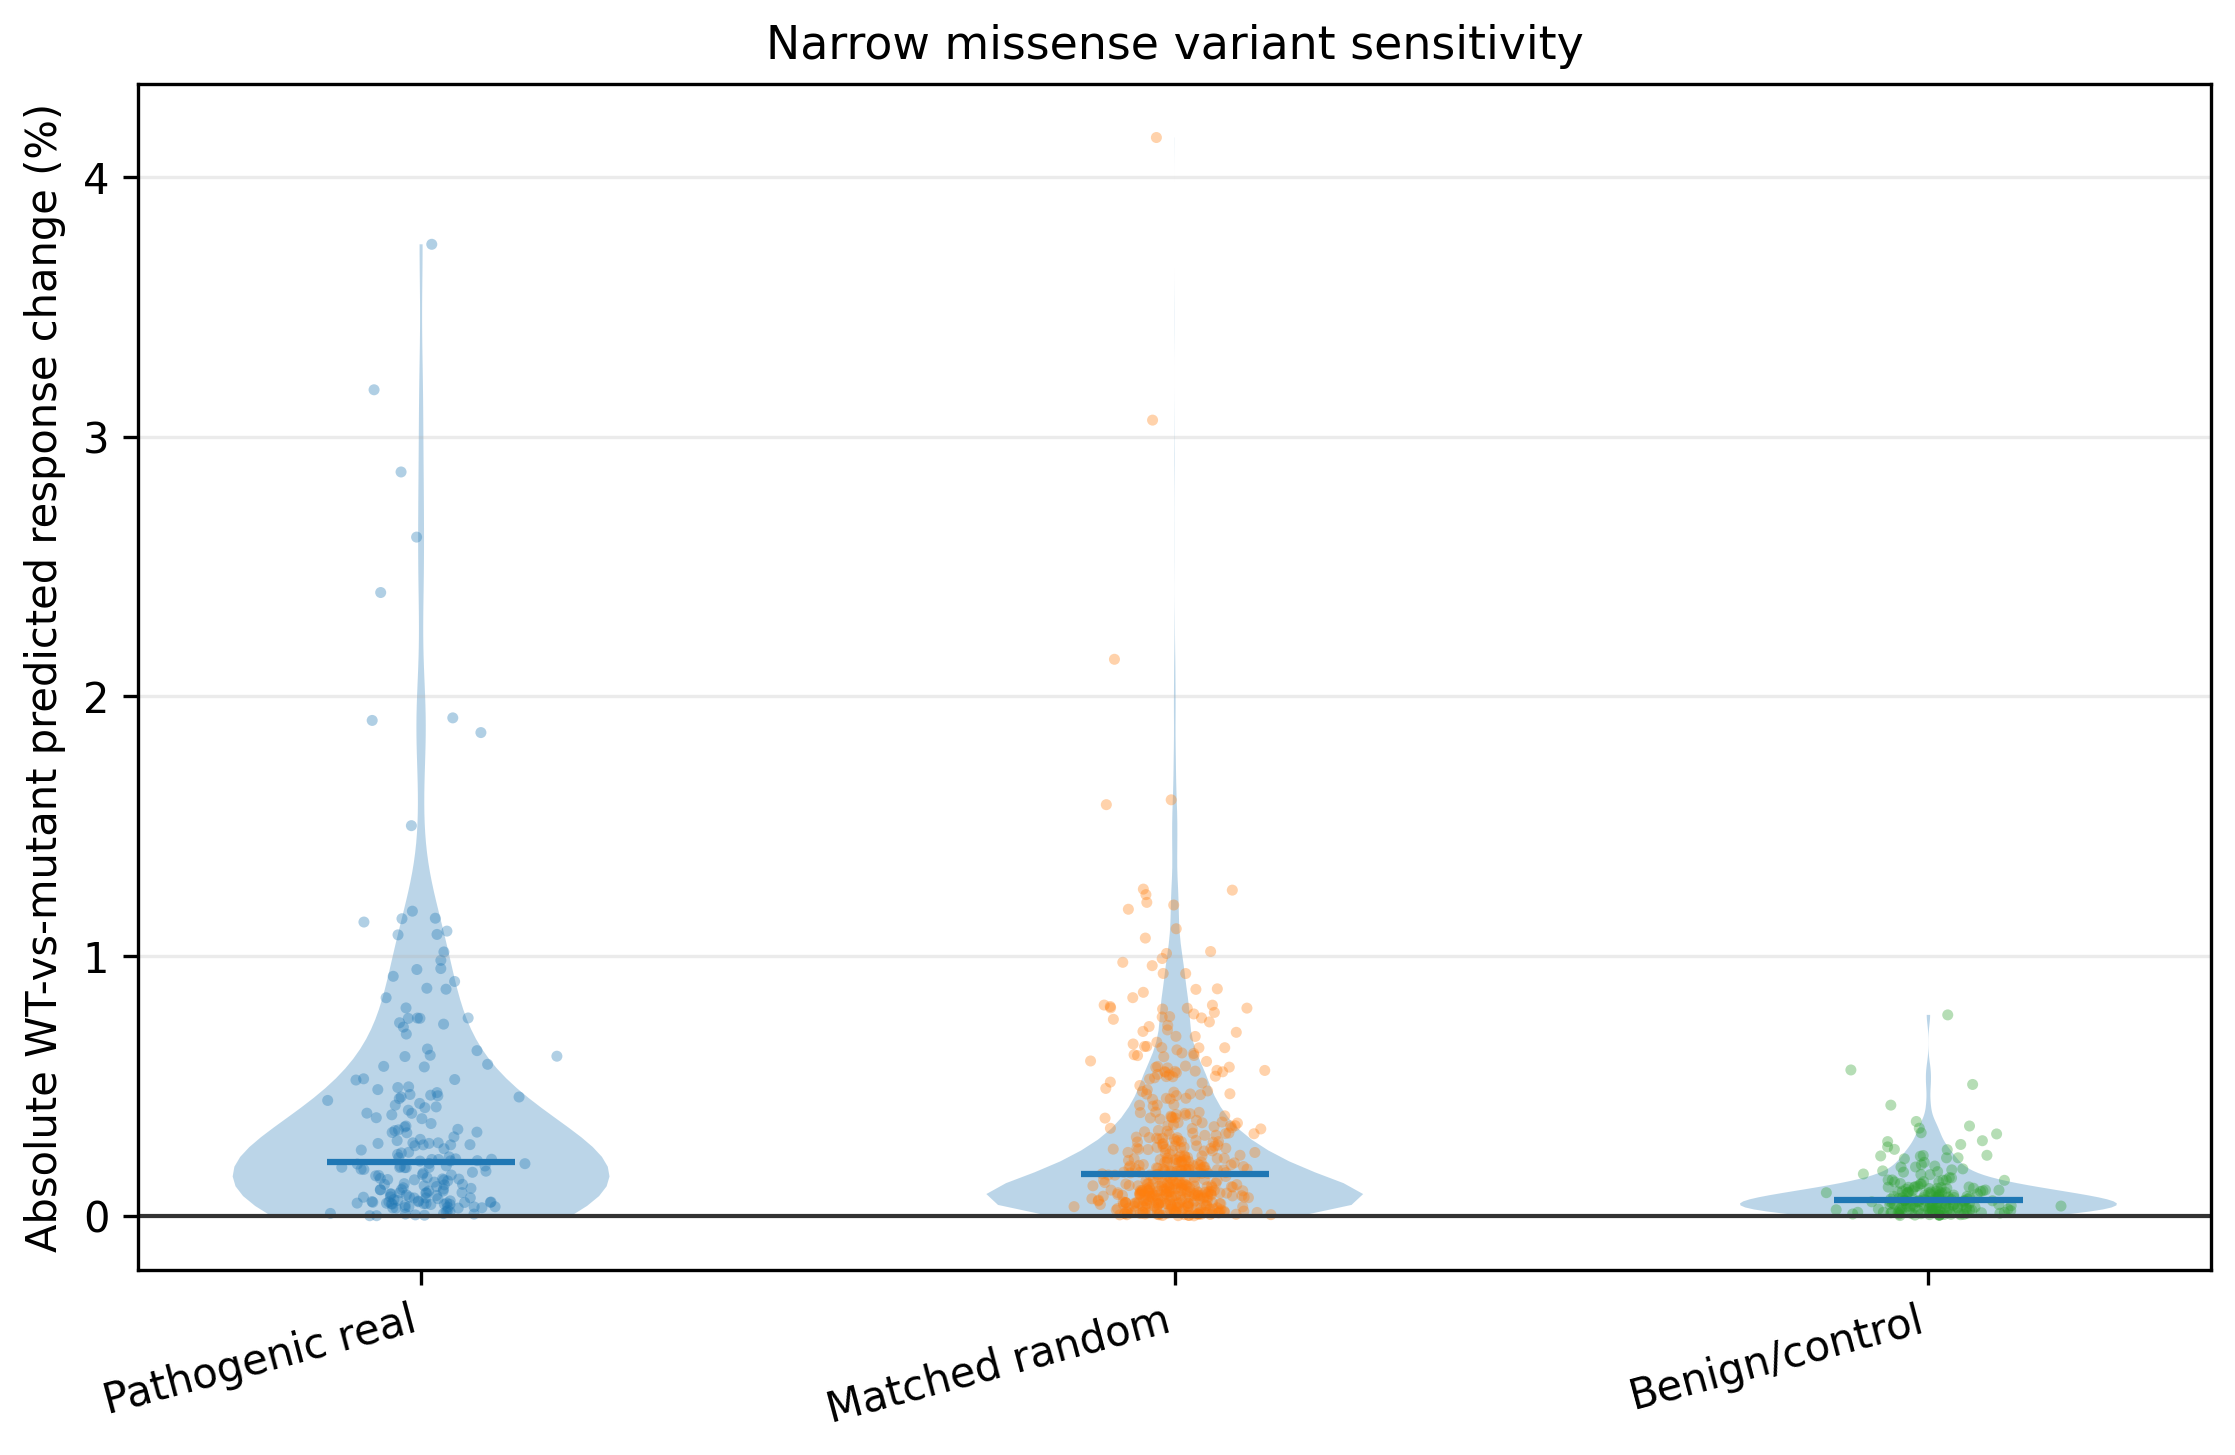
\includegraphics[width=0.84\linewidth]{figures/absolute_variant_effect_violin.png}
\caption{Absolute predicted perturbed cell state activity change for pathogenic variants versus matched controls. This is the primary variant sensitivity framing because damaging TF variants may weaken, strengthen, or redirect predicted response rather than only reducing response magnitude.}
\label{fig:absolute_variant_effect_violin}
\end{figure}

Pathogenic variants produced larger absolute predicted response changes than matched random substitutions, with 189 matched sets, median paired difference 0.0111, and one-sided Wilcoxon \(p=0.0084\). They also produced larger absolute predicted response changes than matched benign/control variants, with 158 matched sets, median paired difference 0.0346, and one-sided Wilcoxon \(p=5.46\times 10^{-6}\). The distributions overlap substantially, so this supports sequence sensitivity, not individual variant classification.

Variants also changed the retrieval distribution over \ag\ entries. Pathogenic variants moved retrieval more than matched random substitutions, with median paired difference \(1.08\times 10^{-4}\) and one-sided Wilcoxon \(p=2.62\times 10^{-4}\). The comparison against matched ClinVar benign variants was weaker and not significant (Table~\ref{tab:matched_retrieval_change}). Thus sequence changes propagate through the retrieval layer, but the retrieval movement should not be interpreted as measured binding-site disruption.

\begin{table}[t]
\centering
\caption{Matched retrieval change diagnostic. Positive paired differences mean pathogenic variants moved the retrieval distribution more than the matched control group.}
\label{tab:matched_retrieval_change}
\resizebox{\linewidth}{!}{%
\begin{tabular}{lccc}
\toprule
\textbf{Comparison} & \textbf{Matched sets} & \textbf{Median paired difference} & \textbf{Wilcoxon \(p\)} \\
\midrule
Pathogenic vs. matched ClinVar benign & 158 & \(4.34\times 10^{-5}\) & 0.2478 \\
Pathogenic vs. matched random substitutions & 189 & \(1.08\times 10^{-4}\) & \(2.62\times 10^{-4}\) \\
\bottomrule
\end{tabular}%
}
\end{table}

\begin{figure*}[t]
\centering

\includegraphics[width=0.95\textwidth]{figures/variant_retrieval_chromosome_diagrams_matched_benign_scarf_1kb.png}
\caption{Variant-specific retrieval movement across \ag\ key entries. Each chromosome is split into visualization bins for the retrieved gene-associated entries used by \hoptf. The panels show wild type, pathogenic mutant, matched benign/control sequence, and pathogenic minus wild type change for selected examples. These are retrieval weights over candidate regulatory context entries, not measured binding sites.}
\label{fig:variant_retrieval_chromosome_heatmap}
\end{figure*}

\subsection{\texorpdfstring{\(\beta\)}{beta} tunes retrieval concentration}

A sweep over retrieval inverse temperature tests whether \hoptf\ behaves like a controllable associative retrieval system. As \(\beta\) increases from 0.1 to 30, retrieval moves from diffuse averaging over nearly all \ag\ key entries toward more focused use of a smaller subset. Median effective retrieved loci fall from \(5.49\times 10^4\) to \(5.21\times 10^3\), while median top-100 mass rises from 0.0019 to 0.2166 (Table~\ref{tab:beta_sensitivity}). Adjacent \(\beta\) values have median top-100 overlap of 1.0, indicating that \(\beta\) mostly sharpens a stable ranking rather than replacing the highest-ranked loci.

\begin{table}[t]
\centering
\caption{\(\beta\) controls retrieval concentration. Effective loci and top-100 mass are medians across TF rows.}
\label{tab:beta_sensitivity}
\begin{tabular}{ccc}
\toprule
\(\beta\) & \textbf{Median effective loci} & \textbf{Median top-100 mass} \\
\midrule
0.1 & \(5.49\times 10^{4}\) & 0.0019 \\
0.3 & \(5.49\times 10^{4}\) & 0.0020 \\
1 & \(5.48\times 10^{4}\) & 0.0023 \\
3 & \(5.37\times 10^{4}\) & 0.0036 \\
10 & \(4.24\times 10^{4}\) & 0.0144 \\
30 & \(5.21\times 10^{3}\) & 0.2166 \\
\bottomrule
\end{tabular}
\end{table}

\begin{figure}[t]
\centering
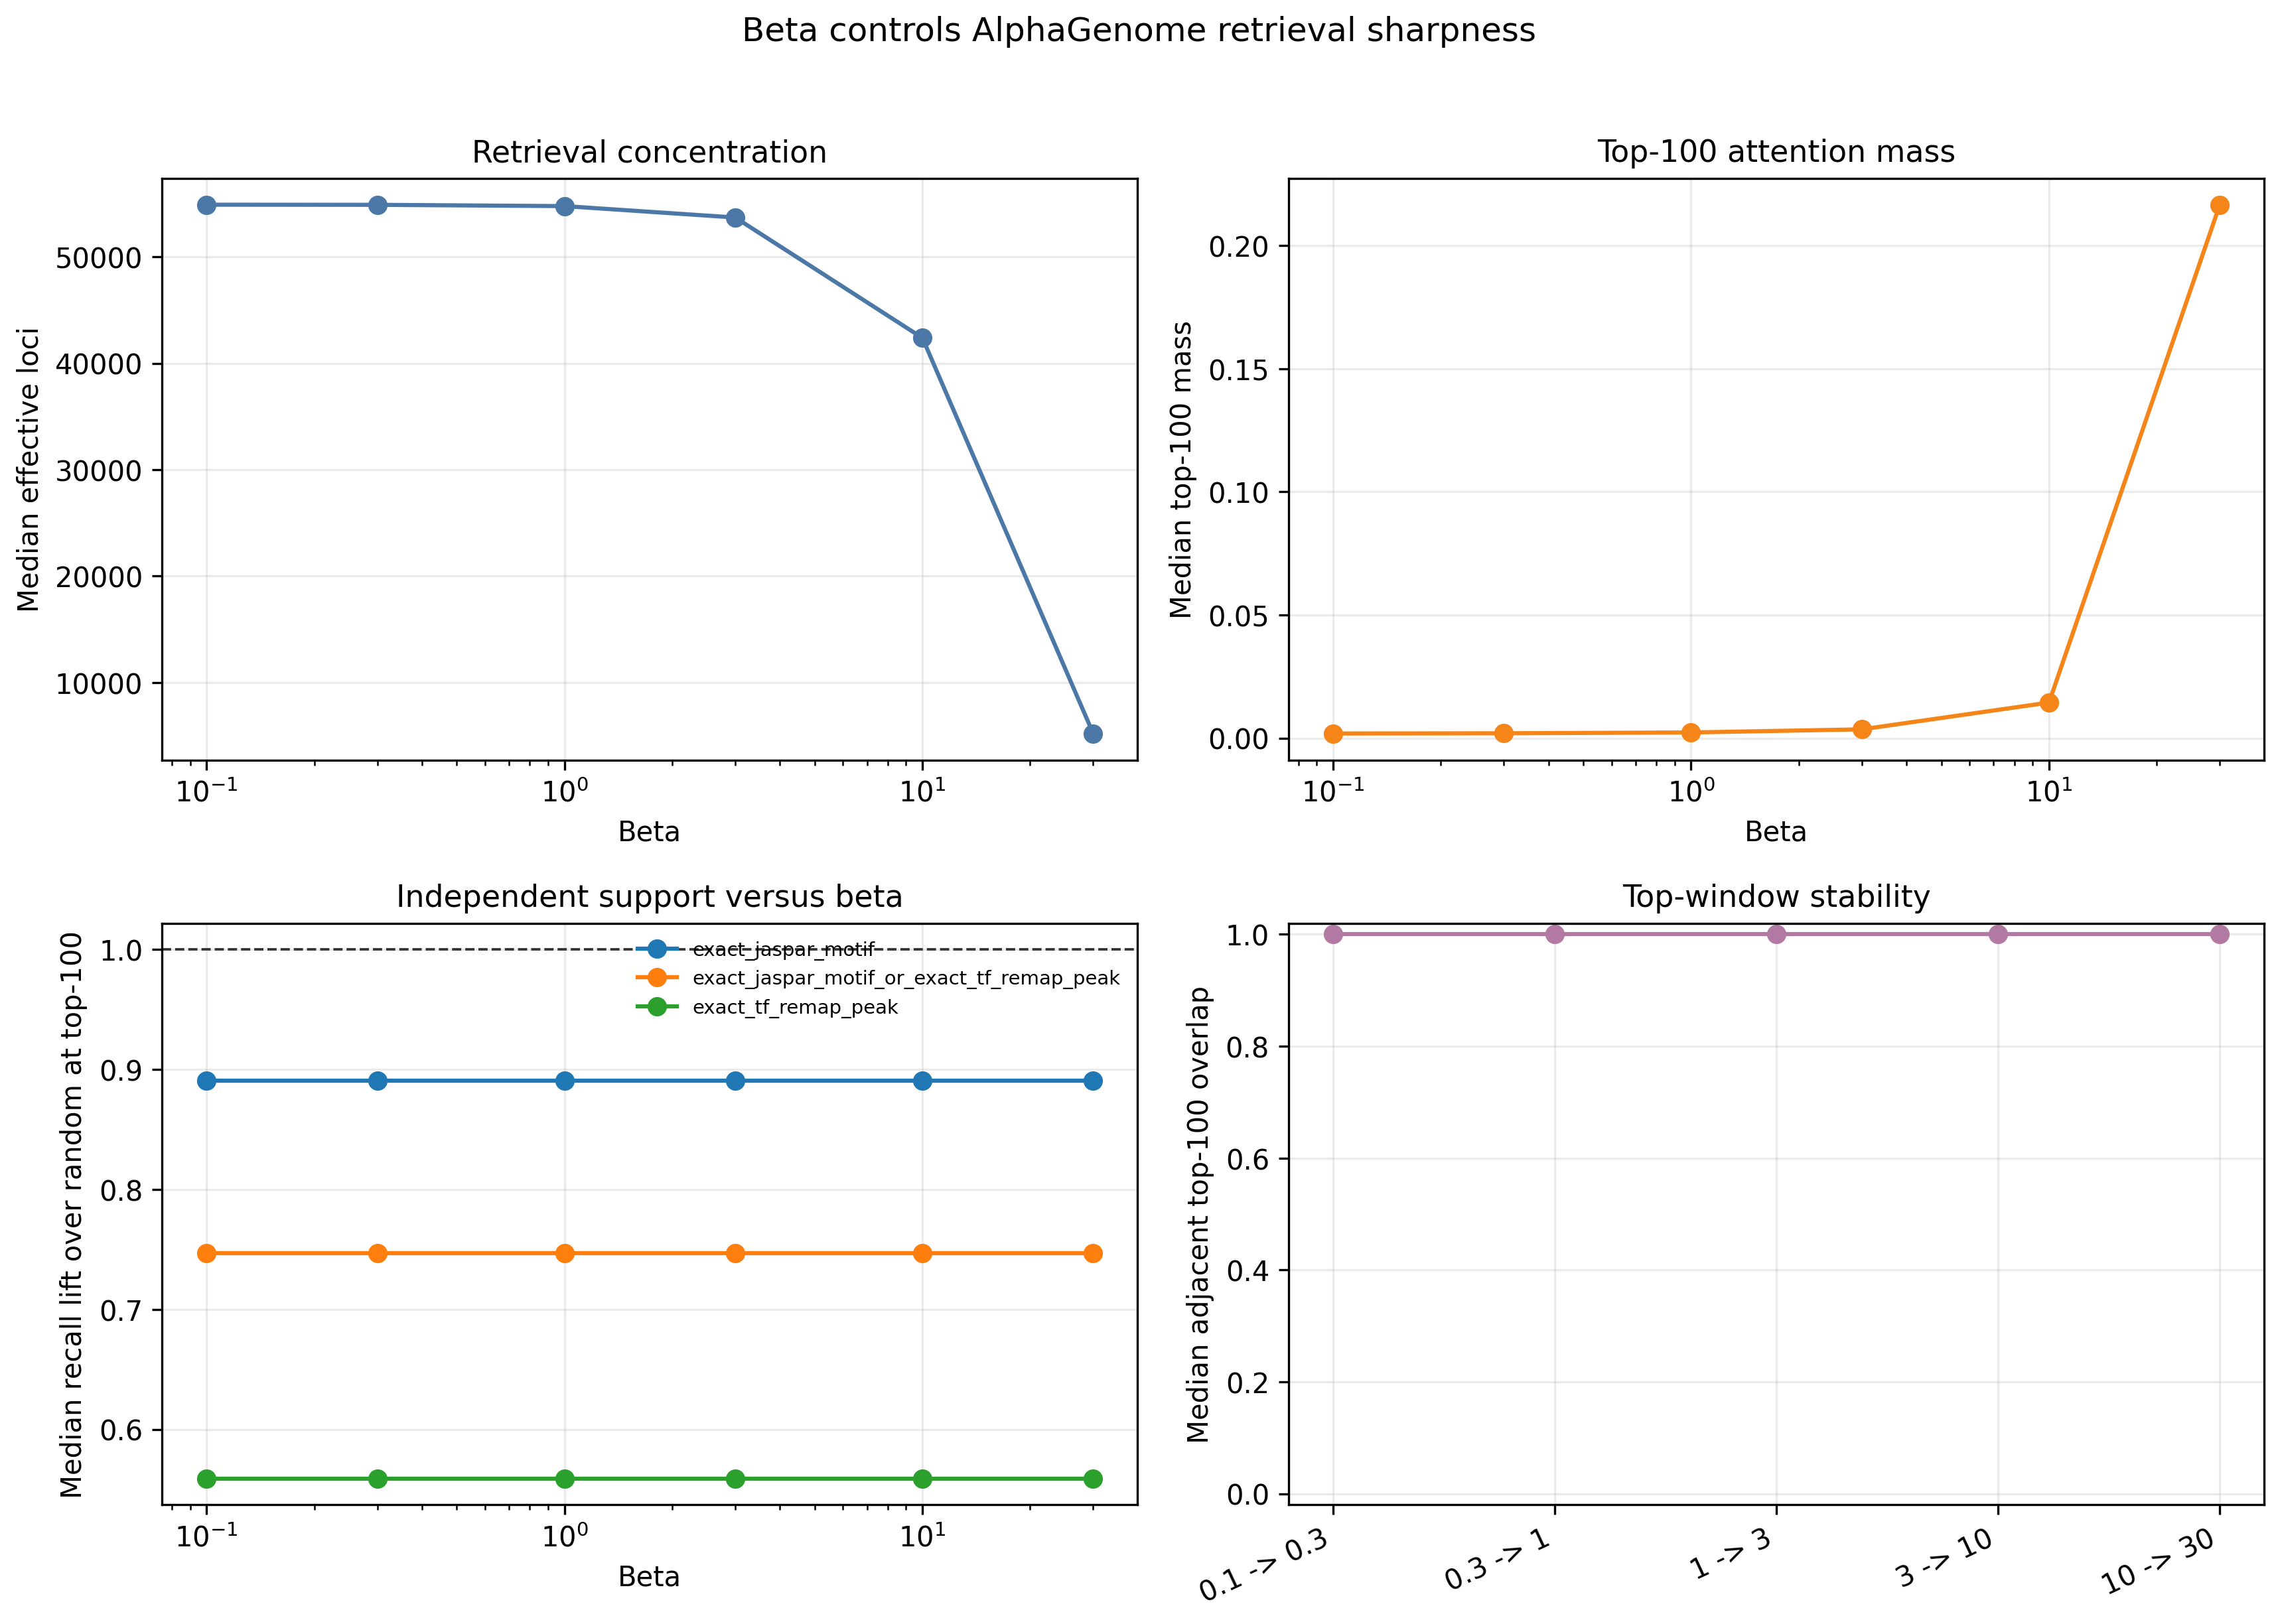
\includegraphics[width=0.9\linewidth]{figures/beta_sweep_figure.png}
\caption{Effect of retrieval inverse temperature \(\beta\). Increasing \(\beta\) shifts retrieval from diffuse averaging over many \ag\ key entries toward more focused use of a smaller subset, while adjacent \(\beta\) values preserve the same top-ranked entries. Independent motif and ReMap support remains weak across the sweep.}
\label{fig:beta_sweep}
\end{figure}

This result supports the intended associative retrieval interpretation: \(\beta\) controls the breadth of regulatory context retrieval. It does not show that \(\beta\) is a dose-calibrated proxy for TF concentration, that higher-\(\beta\) retrieval is more biologically correct, or that any \(\beta\) value improves perturbed cell state prediction.

\subsection{Motif and ReMap support remain weak}

Finally, we tested whether entries with the highest retrieval weights overlap independent motif or binding evidence for the same TF. Motif support uses JASPAR 2024 motif profiles matched by exact TF symbol \citep{rauluseviciute2024jaspar}; external binding support uses ReMap ChIP-seq peaks assigned to the same TF symbol \citep{hammal2022remap}. The validation unit is a 1~kb window centered on the TSS associated with each \ag\ key entry, not an exact motif base or measured binding event.

\begin{table}[t]
\centering
\caption{Motif and ReMap recall remains limited under exact TF symbol matching.}
\label{tab:motif_results}
\resizebox{\linewidth}{!}{%
\begin{tabular}{lcccc}
\toprule
\textbf{Support definition} & \textbf{Top-\(k\)} & \textbf{TF rows} & \textbf{Median recall@\(k\)} & \textbf{Random expectation} \\
\midrule
Exact same-symbol JASPAR motif & 1000 & 1616 & 0.0177 & 0.0182 \\
Exact same-TF ReMap peak & 1000 & 1071 & 0.0113 & 0.0182 \\
Exact JASPAR motif or ReMap peak & 1000 & 1616 & 0.0147 & 0.0182 \\
\bottomrule
\end{tabular}%
}
\end{table}

Under exact TF symbol matching, retrieved entries do not recover a larger fraction of same-TF motif or binding-supported windows than expected under a random ordering of entries. Top-100 support was also modest: the median support fraction was 0.060 for retrieved validation windows and 0.055 for matched background windows, with only 5 TF rows passing FDR \(\leq 0.10\). This is a biological validation limitation, not a positive binding result. The current retrieval distribution can nominate hypotheses, but windows with high retrieval weight remain candidate regulatory contexts rather than validated binding sites.

\begin{figure}[t]
\centering
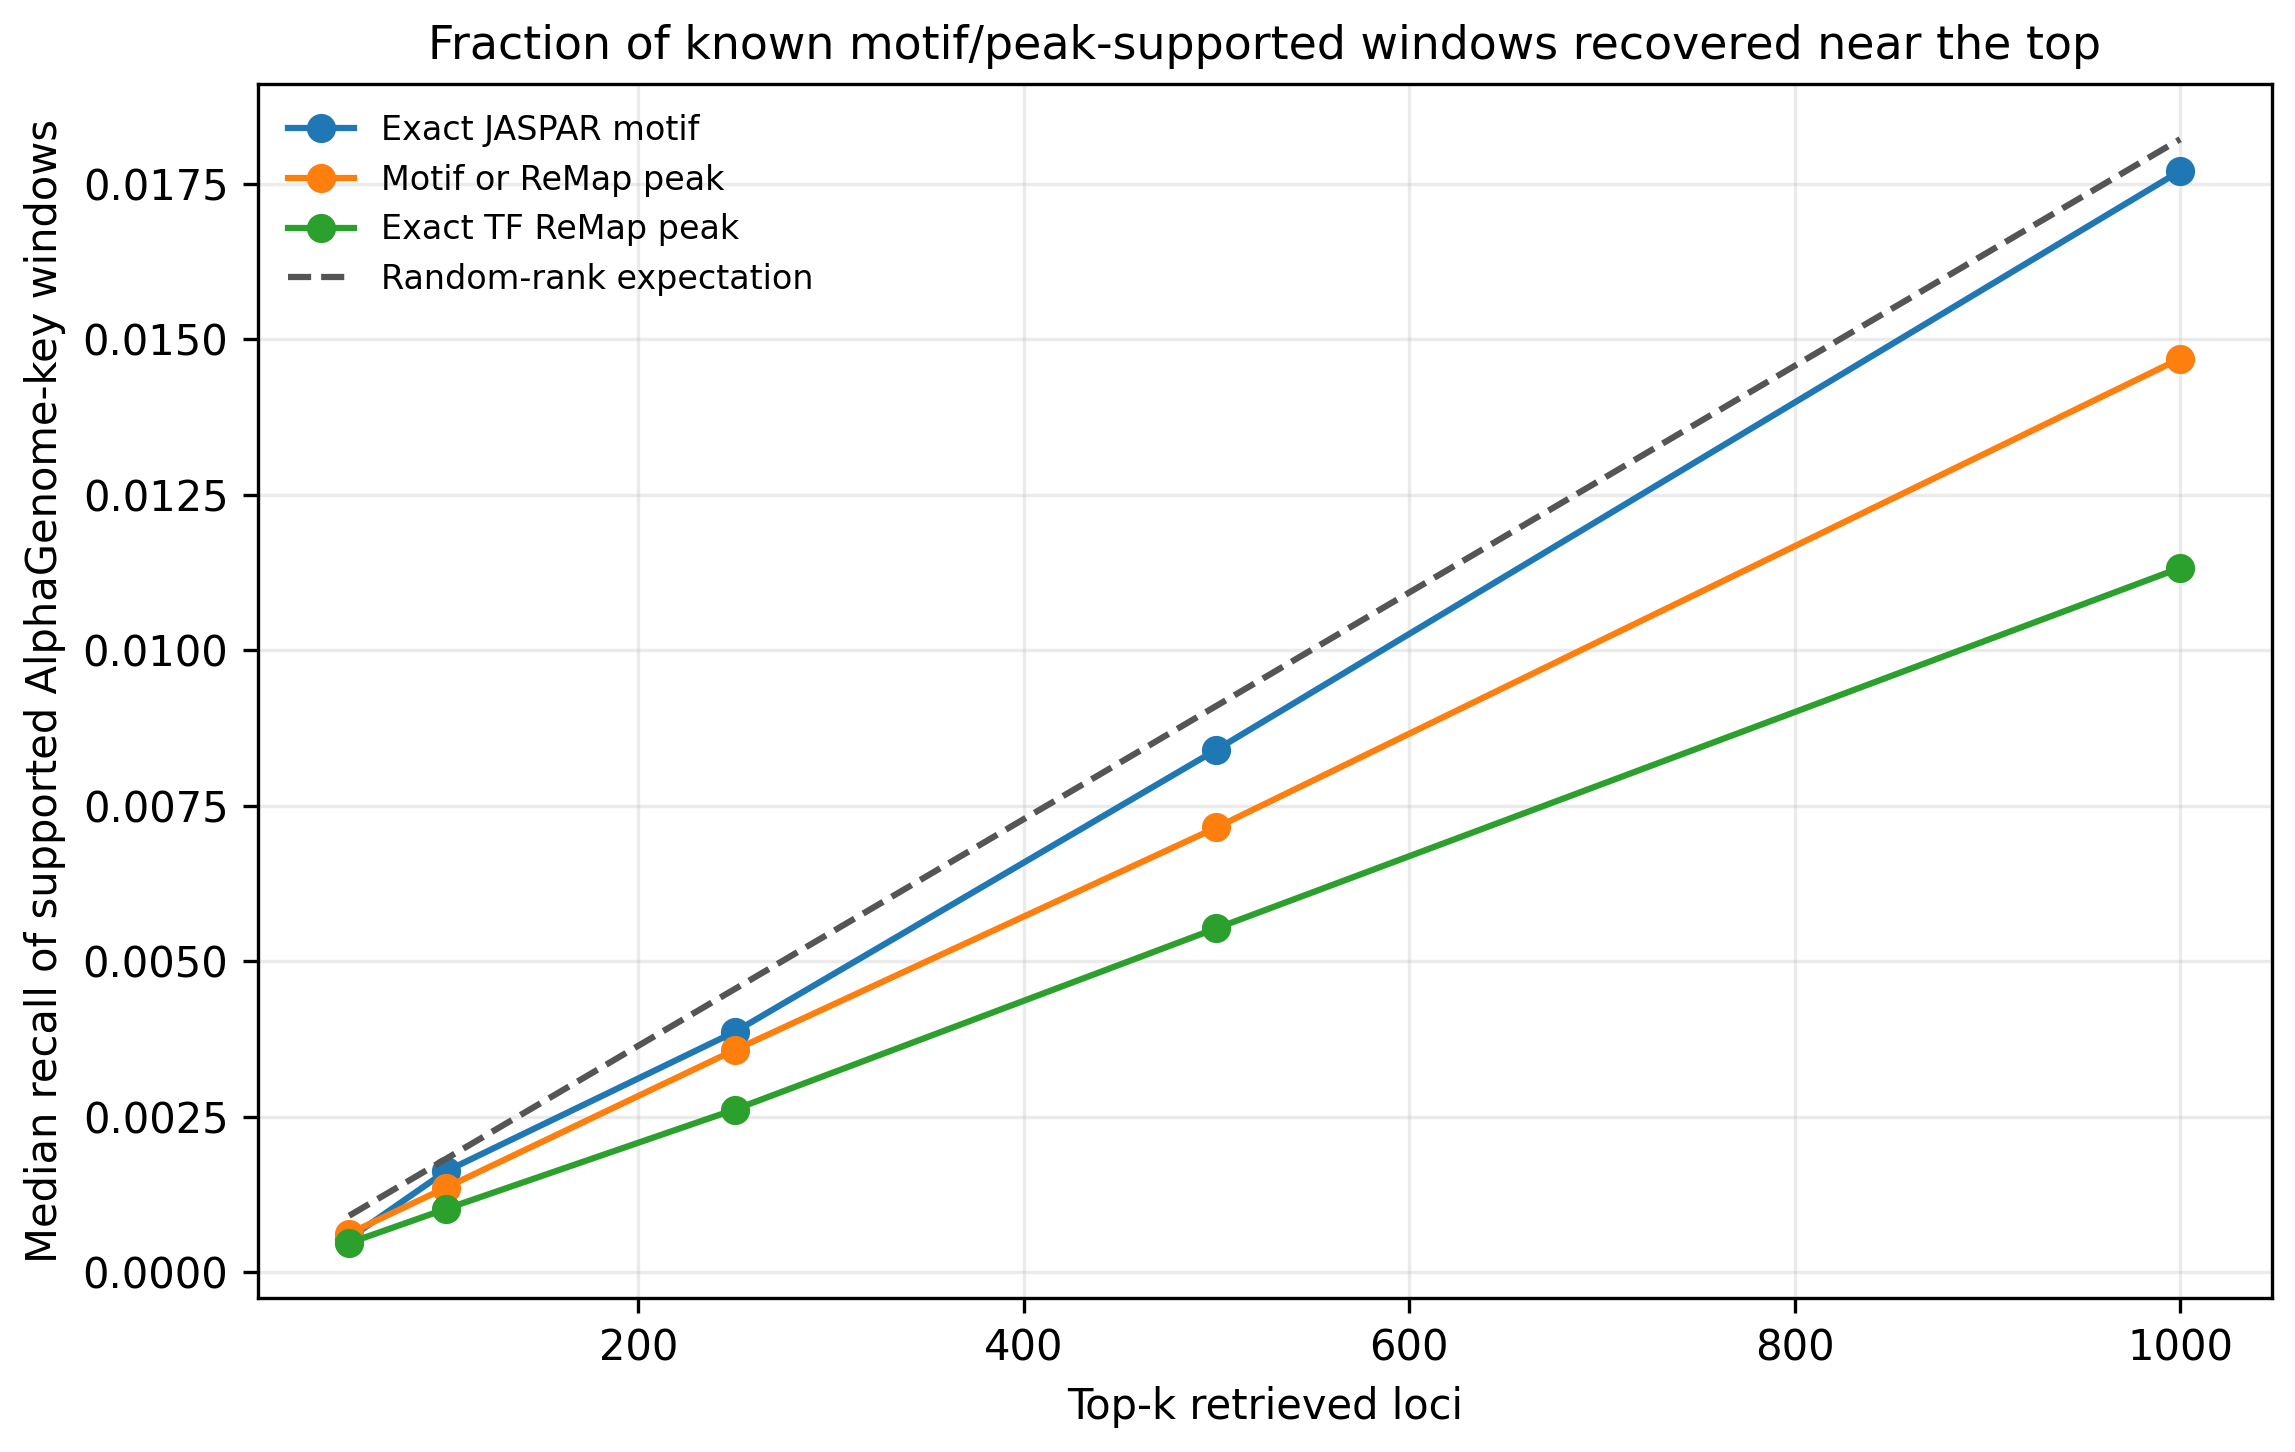
\includegraphics[width=0.86\linewidth]{figures/motif_binding_recall_by_topk.png}
\caption{Recall of exact motif and ReMap support among 1~kb validation windows associated with top retrieved entries. Recall remains near or below the value expected if the retrieval ranking were random at the current validation window scale, so this result should be interpreted as a limitation rather than binding validation.}
\label{fig:motif_binding_recall_by_topk}
\end{figure}

\section{Discussion and Limitations}

\hoptf\ is best interpreted as a model for hypothesis generation. The primary \scarf\ response benchmark is conservative: projected \esm\ is the strongest sequence feature set, but it does not beat protein length, ORF length, and recovered cell count. The stronger positive evidence is narrower: missense variants alter predicted response more than matched controls, sequence changes propagate through retrieval, and \(\beta\) controls retrieval concentration as expected for an associative memory layer.

The main limitations follow directly from this evidence. The model is trained with aggregate perturbation response supervision, not binding labels or causal regulatory labels at locus level. Retrieval weights are therefore candidate scores for regulatory context, not binding probabilities. The response endpoint is frozen \scarf\ latent space; we do not decode predictions to gene expression or claim target recovery at gene level. The reported retrieval analyses use a shared unmasked memory derived from \ag, so they should not be interpreted as accessible region prediction for specific cell types. Exact-symbol motif and ReMap validation is weak at the current 1~kb window scale.

This weak exact-symbol validation should be interpreted in light of the resolution of the retrieval object. TF motifs are short sequence patterns, often on the order of tens of bases, while the diagnostic maps gene-associated \ag\ entries to 1~kb validation windows. A retrieved window can therefore contain a broad regulatory neighborhood rather than the precise base-pair footprint of direct TF binding. Exact TF-symbol matching is also narrow: TFs from related DNA-binding domain families can share sequence preferences, and an \esm-derived protein query may capture family-level compatibility that is not counted by same-symbol motif or ReMap overlap. Finally, because supervision comes from aggregate transcriptomic response, the model can assign weight to downstream functional mediators or response-associated regulatory neighborhoods rather than only primary physical docking sites. High-retrieval loci should therefore be read as functional regulatory hypotheses prioritized by the model, not as in silico ChIP peaks.

These limitations also define the next steps. Retrieval aware of cell state should incorporate cluster-level accessibility priors, predicted accessibility biases, or hard masks where supported by data. Biological validation should move beyond exact-symbol checks by incorporating TF-family support, alias handling, accessibility, enhancer-gene linking, and matched background enrichment.

\section{Future Work}

The most important modeling extension is to train directly on multiple sequence instances per TF isoform rather than using variants only as post hoc perturbations. In such a multiple-instance formulation, the reference isoform and high-confidence tolerated or benign sequence variants would share the same observed TF Atlas response label. The model would then be encouraged to learn retrieval and response predictions that are stable to tolerated sequence variation while remaining sensitive to damaging variants held out for evaluation.

This experiment is future work, not a completed result in this submission. Its success criterion should be two-sided: tolerated/control instances should stabilize or improve held-out response prediction relative to training on reference sequences only, while pathogenic variants should still produce larger absolute response or retrieval changes than tolerated instances. Tier 5 fallback controls should be excluded from the primary claim or reported separately because they lack independent tolerance evidence. This would test the intended distinction between tolerance-aware invariance and loss of sequence sensitivity.

\section{Conclusion}

\hoptf\ frames TF perturbation modeling as sequence-conditioned associative retrieval over a genome-indexed regulatory memory. The current evidence does not justify a broad predictive performance claim, but it does support a narrower and useful conclusion: the retrieval layer is sequence sensitive, its concentration is controllable, and its outputs are auditable hypotheses. The next version of the model should therefore focus on stronger retrieval informed by cell state and biological validation before treating prioritized loci as causal regulatory mechanisms.

\section{Code and Data Availability}

Code is available in the public GitHub repository at \url{https://github.com/cpudan/HopTF}. Public data artifacts, manifests, and reusable outputs are hosted on Hugging Face at \url{https://huggingface.co/datasets/pvd232/HopTF}. The dataset repository is organized as an artifact store rather than a single homogeneous tabular dataset, so reproducibility should follow the file paths and manifests documented there.

\bibliographystyle{icml2026}
\bibliography{references}

\newpage
\appendix
\onecolumn

\section{Related Work Details}
\label{app:related_work}

Classical Hopfield networks introduced content-addressable associative memory: stored patterns can be retrieved from partial or noisy cues through energy-based dynamics \citep{hopfield1982}. Dense associative memory generalized this idea to higher-capacity energy functions capable of storing and retrieving many more patterns \citep{krotov2016}. Modern Hopfield networks extend associative memory to continuous states and show that the update rule is equivalent to the attention mechanism used in transformers \citep{ramsauer2021,vaswani2017}. In \hoptf, the stored patterns are genomic locus embeddings, the cue is a TF isoform embedding, and the retrieved state is a regulatory context vector used to predict perturbation response.

This perspective has already been useful in biological multiple-instance learning. DeepRC uses transformer-like attention, equivalently modern Hopfield retrieval, to classify immune repertoires from extremely large bags of immune receptor sequences with sparse disease-associated witnesses \citep{widrich2020}. The analogy to \hoptf\ is direct but not identical. In immune repertoire classification, the model must identify a small set of disease-relevant sequences from a massive repertoire. In \hoptf, the model must identify TF-compatible regulatory contexts from a large set of genomic loci using only aggregate transcriptional response supervision.

Single-cell perturbation response methods such as GEARS, CellOT, and scGPT address related prediction problems \citep{roohani2023,bunne2023,cui2024}. Mechanistic approaches such as CellOracle and SCENIC+ integrate motifs, accessibility, enhancer-gene links, and regulatory networks \citep{kamimoto2023,gonzalezblas2023}. Protein-aware TF-DNA binding models such as TransBind and TFBindFormer condition local DNA binding predictions on protein representations \citep{basnet2026,liutfbindformer2026}. STRAND is a close conceptual neighbor because it models sequence-conditioned single-cell transport, but it conditions on regulatory DNA sequence at the intervention locus, whereas \hoptf\ queries a regulatory memory using TF protein sequence \citep{fu2026}. Together, these comparisons define \hoptf's scope: it is not a replacement for GRN simulators, local binding classifiers, or generic perturbation predictors; it tests whether protein sequence can query regulatory context derived from genome features in a way that remains auditable.

\section{Detailed Method Variants}
\label{app:detailed_methods}

\subsection{Problem formulation}

Let \(x \in \mathbb{R}^G\) denote a single-cell expression vector over \(G\) genes. Let \(p\) index a TF perturbation, and let \(s_p\) denote the amino acid sequence of the perturbed TF isoform. The training data consist of control cells and cells after TF perturbation. For each TF \(p\), we observe samples from a control distribution \(P_0\) and a perturbed distribution \(P_p\), but we do not observe which genomic loci mediate the perturbation response.

The downstream goal is to learn a conditional vector field that transports control cell latents \(z_0\) toward perturbed latents \(z_1 \sim P_p\):
\begin{equation}
    \frac{d z_t}{dt} = v_\theta(z_t, t, z_0, \mu_{0p}), \qquad t \in [0,1],
\end{equation}
where \(\mu_{0p}\) is a perturbation representation conditioned on TF sequence and cell state, produced by associative retrieval over genomic loci. The latent locus activation distribution is
\begin{equation}
    \alpha_{0pi} = P_\theta(i \mid z_0, s_p), \qquad i = 1,\ldots,N.
\end{equation}
The model is not trained with labels for \(\alpha_{0pi}\). Instead, \(\alpha_{0pi}\) is induced by the perturbation transport objective. This is the weakly supervised multiple-instance structure: the bag is the candidate locus set, the query is the TF isoform sequence, and the bag-level target is the aggregate transcriptional response.

\subsection{Foundation features and query construction}

In the current implementation, \esm\ \citep{evolutionaryscale2024} uses the 600M-parameter model with mean pooling over non-special tokens, producing a frozen 1152-dimensional isoform embedding. The encoder ablation also tested \esmdbp, a DBP-specialized ESM2-style 650M model from ESM-DBP \citep{zeng2024esmdbp}, with mean pooling over non-special tokens into a frozen 1280-dimensional embedding. The \esmdbp\ embedding pass covered 3264 of 3548 vocabulary entries; 284 entries had no local amino acid sequence and 139 sequences were truncated to the 1022-token model limit. Missing sequence rows are retained in the aligned vocabulary with a mask, so downstream baselines can distinguish unavailable sequence information from real zero-valued embeddings.

The \ag\ memory bank is fixed after loading the gene-pooled archive. We do not fine-tune \ag, adapter-tune the key/value memory, or add residual memory updates \(\Delta k_i,\Delta v_i\). The trained components are lightweight task-specific projections and predictors built on top of frozen features: the projection from protein embedding to \ag\ key space used to form Hopfield queries, ridge or small neural predictors used in endpoint benchmarks, and conditional vector field parameters in the earlier PCA endpoint transport analyses.

\subsection{Cell state modulation and retrieval masks}

The most conservative base model uses no mask specific to cell state:
\begin{equation}
    r_{pi} = \beta q_p^\top k_i.
\end{equation}
A version conditioned on cell state could add a retrieval bias or mask derived from the cell latent \(z_0\):
\begin{equation}
    r_{0pi} = \beta q_p^\top k_i + b_\eta(z_0, h_i^{\mathrm{AG}}),
\end{equation}
where \(b_\eta\) may represent a learned compatibility score between cell state and locus, an accessibility prior by cluster, or a log-accessibility mask. If \(m_i(z_0) \in \{0,1\}\) denotes a hard accessibility mask, this can be written as
\begin{equation}
    r_{0pi} =
    \begin{cases}
        \beta q_p^\top k_i, & m_i(z_0)=1,\\
        -\infty, & m_i(z_0)=0.
    \end{cases}
\end{equation}
In practice, hard masks for each cell may be unstable or unrealistic if accessibility is not observed for every target cell. An accessibility bias by cluster or cell type may be a more robust intermediate design:
\begin{equation}
    r_{cpi} = \beta q_p^\top k_i + \lambda A_{ci},
\end{equation}
where \(c\) is a cluster in \scarf\ latent space and \(A_{ci}\) is an availability prior for locus \(i\) in cluster \(c\).

\subsection{Conditional flow endpoint}

The retrieved representation \(\mu_{0p}\) conditions a time-dependent vector field in cell state latent space:
\begin{equation}
    \frac{d z_t}{dt} = v_\theta(z_t, t, z_0, \mu_{0p}).
\end{equation}
In the flow-matching variant of \hoptf, training uses conditional flow matching with minibatch optimal transport couplings \citep{tong2024cfm,tong2024sf2m}. For a TF perturbation \(p\), let \((z_0,z_1)\) be a paired sample from a minibatch OT coupling between control latents and perturbed latents. For \(t \sim \mathrm{Uniform}(0,1)\), define
\begin{align}
    z_t &= (1-t)z_0 + t z_1, &
    u_t &= z_1-z_0.
\end{align}
The flow matching objective is
\begin{equation}
    \mathcal{L}_{\mathrm{CFM}} =
    \mathbb{E}_{p,(z_0,z_1),t}\left[
    \left\|v_\theta(z_t,t,z_0,\mu_{0p}) - (z_1-z_0)\right\|_2^2
    \right].
\end{equation}
For the final response analyses, the endpoint representation is frozen \scarf\ response space. Earlier PCA endpoint transport analyses used a separate 50-dimensional PCA centroid target and integrated a conditional vector field from the control mean; those PCA results are retained as sensitivity evidence rather than the primary response representation.

\section{Extended Evaluation Design}
\label{app:comparison_design}

\subsection{Data setup and splits}

The main perturbation data come from TF Atlas of directed differentiation, which profiles TF isoform overexpression in H1 hESCs at single-cell resolution \citep{joung2023}. The local TF Atlas subset backed by \scarf\ contains 671,453 cells by 37,528 genes, with 3,266 unique perturbation labels in the cell metadata. It includes 1,000 GFP control cells and 1,000 mCherry control cells. Perturbation labels in the h5ad exactly match the HopTF perturbation metadata used for the controlled sequence feature analyses.

The analyses use the staged TF Atlas subsample and its precomputed \scarf\ embeddings rather than rerunning cell-level quality control from raw reads. Perturbation metadata are joined by perturbation identifier and must include recovered cell count, protein length, ORF length, gene symbol, isoform identifier, and isoform embedding identifier. Fitted benchmarks and retrieval diagnostics exclude perturbation rows with fewer than five recovered cells when they use the shared HopTF modeling scripts. The main train/test evaluation is grouped by TF gene symbol, not by random cells, so isoforms or variants from the same gene do not leak across held-out folds.

For the \scarf\ response target, GFP and mCherry control cells are pooled to form a single control reference mean. We did not perform batch-matched control selection in the reported \scarf\ benchmark. Primary \scarf\ MSE and cosine metrics are computed in latent response space. Endpoint metrics standardized by controls are reported only for the earlier PCA transport sensitivity analyses or where explicitly labeled; they are not decoded gene expression metrics.

\subsection{Full comparison design}

\begin{table}[t]
\centering
\caption{Planned comparisons and their purpose.}
\label{tab:comparisons}
\begin{tabular}{p{0.24\linewidth}p{0.38\linewidth}p{0.28\linewidth}}
\toprule
\textbf{Comparison} & \textbf{Description} & \textbf{Question tested} \\
\midrule
Control / no-perturbation & Predict no movement from control latent. & Is any perturbation modeling learned? \\
Average TF effect & Use the mean perturbation shift across training TFs. & Are gains TF-specific or just average response? \\
TF ID embedding & Replace protein sequence with a learned TF identity embedding. & Does protein sequence add value? \\
ESM-only flow & Condition flow on TF protein embedding without genomic memory retrieval. & Does locus retrieval add value beyond protein sequence? \\
Random / shuffled memory & Replace \ag\ loci with random or shuffled locus embeddings. & Does regulatory memory carry useful signal? \\
Shuffled TF sequence & Query memory using shuffled or mismatched TF embeddings. & Are retrieval weights TF-specific? \\
No cell state bias & Remove accessibility bias by cell state or cluster. & Does cell context matter? \\
Length / ORF / cell-count inputs & Predict from sequence length, ORF length, and perturbation cell count. & How much can these measured quantities explain? \\
\bottomrule
\end{tabular}
\end{table}

The implemented comparison set is narrower than the full design table. For perturbed cell state prediction, we compare protein length plus ORF length plus recovered cell count, raw \esm, raw \esmdbp, \esm\ projected into \ag\ key space, \esmdbp\ projected into \ag\ key space, Hopfield query features, and shuffled sequence controls where available. The primary \scarf\ benchmark also tests whether adding projected or raw \esm\ features improves over the length/ORF/cell-count covariate model. We did not complete a learned TF-ID embedding baseline, a fully random memory baseline for the primary \scarf\ benchmark, a cell state accessibility bias ablation, or decoded gene expression comparisons.

\subsection{Retrieval and biological validation metrics}

We evaluate the locus activation distribution independently of perturbed cell state prediction using retrieval entropy \(H(\alpha)\), effective number of loci \(N_{\mathrm{eff}}\), top-\(k\) mass, \(\beta\) sensitivity, motif support among top retrieved loci, overlap with external ChIP-seq peaks where available, and retrieval movement under variants. The implemented biological support diagnostics use 1~kb TSS-centered validation windows assigned to \ag\ key entries. Per-TF enrichment tests use Fisher exact tests for support in retrieved versus matched background windows, with Benjamini-Hochberg FDR correction and FDR \(\leq 0.10\) reported as the exploratory threshold.

\section{Benign and Control Variant Construction}
\label{app:variant_controls}

The benign/control table is constructed as a control set tiered by evidence for the local HopTF isoforms, not as a claim that every row is molecularly neutral for TF function. We start from all 3,264 non-control TF isoforms in the local TF Atlas perturbation metadata and create two frozen natural evidence artifacts: an uncapped table containing all currently mapped ClinVar, gnomAD, and MaveDB rows \citep{landrum2025clinvar,karczewski2020gnomad,esposito2019mavedb}, and a capped table containing up to 10 natural benign/control candidates per isoform. Natural human evidence is always used before any synthetic control rows.

Natural variants are accepted only after exact protein coordinate checking against the local HopTF isoform sequence. The reference amino acid at the one-based variant position must match the local wild-type sequence, and the mutant protein sequence is regenerated from the local sequence rather than copied from the source table. We exclude rows with ambiguous coordinate mapping, non-missense changes, conflicting or uncertain clinical labels, pathogenic or likely pathogenic annotations in the control set, and source records without the information needed to reproduce the protein substitution. Each retained row stores both formal HGVS protein notation, such as \texttt{p.Arg339Gln}, and one-letter shorthand notation, such as \texttt{R339Q}; all HGVS strings in the frozen tables were parsed and sequence checked.

\begin{table}[t]
\centering
\caption{Benign/control evidence tiers used for variant control construction. Selected rows are the rows used in the regenerated capped table with 10 rows per isoform.}
\label{tab:benign_control_tiers}
\resizebox{\linewidth}{!}{%
\begin{tabular}{llcc}
\toprule
\textbf{Tier} & \textbf{Inclusion rule} & \textbf{Uncapped rows} & \textbf{Selected rows} \\
\midrule
Tier 1 & Clinical benign/control: ClinVar benign, likely benign, or benign/likely benign; no conflicts; exact local isoform match & 2,064 & 1,817 \\
Tier 2a & Strong population-tolerated: gnomAD v4.1 exome missense row; no disease/conflict annotation; exact local isoform match; group-maximum AF at least 1\% & 2,734 & 2,065 \\
Tier 2b & Moderate population-tolerated: gnomAD v4.1 exome missense row passing staged population-tolerance filters but below strong threshold & 4,789 & 1,940 \\
Tier 3 & Functional assay control: MaveDB assay row with a high function score; exact local isoform match; unambiguous high-score-as-more-functional convention; no local ClinVar deleterious match & 132 & 67 \\
Tier 4 & Ortholog-supported synthetic control: alternate residue is observed at the aligned position in an Ensembl Compara ortholog; conservative chemistry and local sensitive position filters pass; Pfam domain architecture matches & -- & 18,600 \\
Tier 5 & Legacy conservative fallback control: deterministic conservative substitution used only when Tiers 1--4 do not provide enough rows for the fixed file with 10 rows per isoform & -- & 8,151 \\
\bottomrule
\end{tabular}%
}
\end{table}

\begin{figure}[t]
\centering
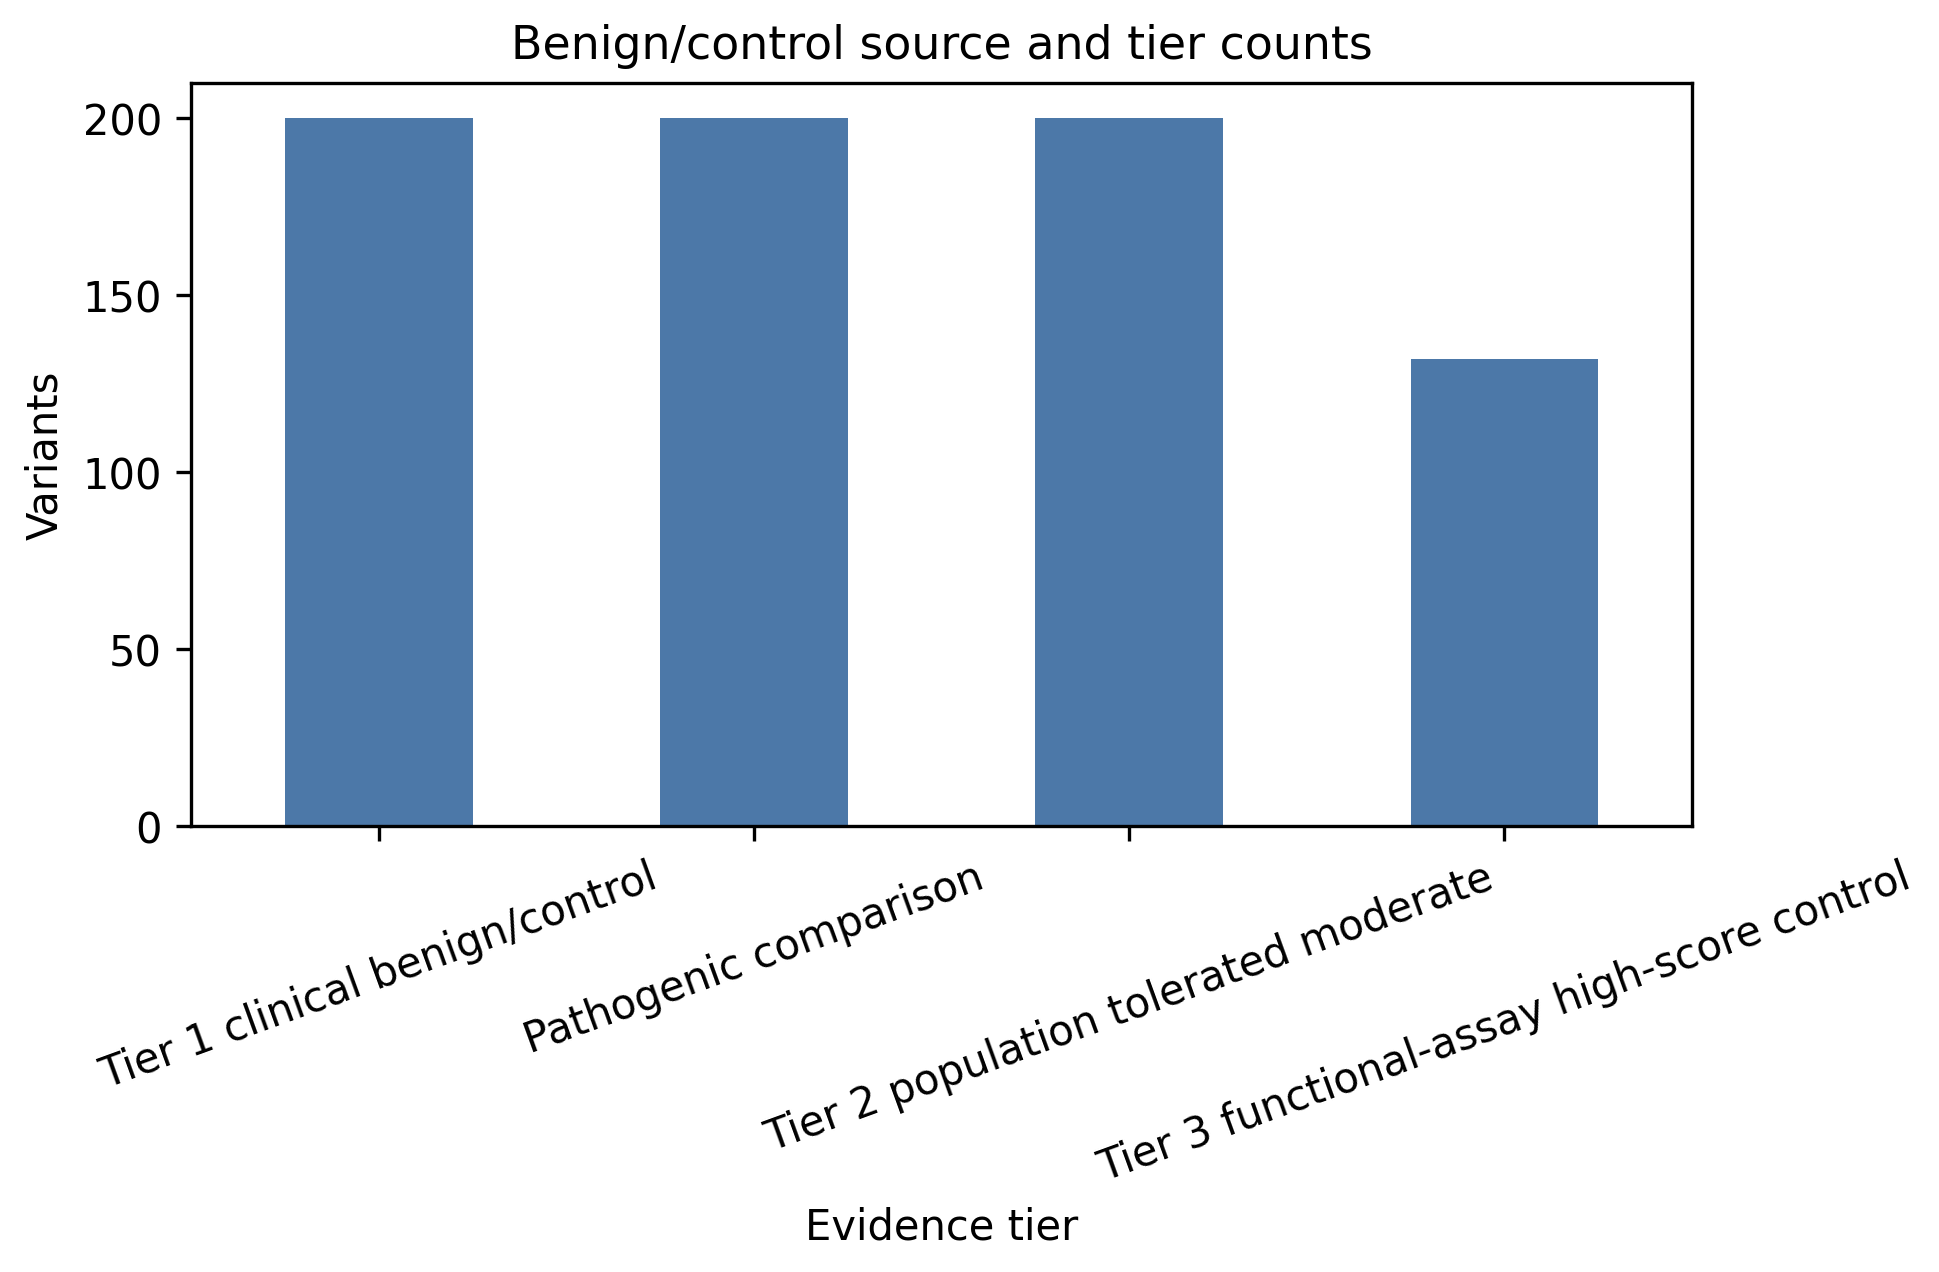
\includegraphics[width=0.7\linewidth]{figures/benign_control_tier_counts.png}
\caption{Composition of the benign/control variant panel tiered by evidence. Natural clinical, population, and functional assay evidence is prioritized first; tolerated substitutions supported by ortholog evidence fill many remaining fixed size slots; legacy conservative fallback controls are retained only where needed for exactly 10 variants per TF isoform.}
\label{fig:benign_control_tier_counts}
\end{figure}

The natural evidence table contains 9,719 rows across 717 isoforms; 435 isoforms have at least 10 natural rows. Because most TF isoforms currently have fewer than 10 natural benign/control rows, we stage a separate tier of synthetic controls supported by ortholog evidence rather than filling the table directly with arbitrary conservative substitutions. For this tier, each proposed mutant residue must be observed at the corresponding aligned position in a non-human Ensembl Compara ortholog \citep{dyer2025ensembl}. The ortholog protein is aligned back to the local HopTF isoform sequence, the local wild-type residue must match the proposed one-based position, and the mutant sequence is regenerated from the local HopTF sequence. The candidate must pass conservative amino acid chemistry filters and avoid sequence edges, C2H2-like zinc-finger motifs, basic patches, leucine-zipper-like heptads, low-complexity windows, and cysteine, histidine, glycine, proline, or tryptophan positions when possible. In the final frozen control construction, we additionally scan the human and ortholog proteins with Pfam \citep{mistry2021pfam} and require the same Pfam domain architecture tuple before accepting the substitution supported by ortholog evidence.

The ortholog-supported generator produced 22,551 candidate substitutions across 2,554 isoforms, with 2,039 isoforms reaching 10 controls supported by ortholog evidence. In the regenerated capped table, natural evidence is selected first, then ortholog-supported tier 4 rows fill the next slots, and tier 5 legacy conservative fallback rows are used only for remaining slots needed to preserve exactly 10 variants for every isoform. The capped table contains 32,640 rows: 5,889 natural evidence rows, 18,600 ortholog-supported tier 4 rows, and 8,151 tier 5 fallback rows. A total of 2,259 isoforms need no tier 5 fallback.

Tier 4 rows are reported as \emph{tolerated substitutions supported by ortholog evidence} or \emph{evolutionarily supported synthetic controls}. They are not clinical benign variants and are not treated as direct evidence of molecular neutrality. Tier 5 rows are conservative fallback controls. They have no independent clinical, population, functional, or ortholog evidence, and they are included only when Tiers 1--4 do not provide enough rows to maintain the fixed design of 10 control substitutions per TF isoform.

\section{PCA Sensitivity and Encoder Diagnostics}
\label{app:pca_sensitivity}

\subsection{Older PCA latent benchmark}

The older PCA latent benchmark asked whether a TF sequence representation helps predict perturbed cell state after protein length, ORF length, and recovered cell count are included. It is retained as sensitivity evidence, not the main predictive claim.

\begin{table}[t]
\centering
\caption{PCA latent perturbed cell state prediction on grouped held-out-gene splits. Lower MSE is better.}
\label{tab:perturbed_state_results}
\resizebox{\linewidth}{!}{%
\begin{tabular}{lccc}
\toprule
\textbf{Feature set} & \textbf{MSE} & \textbf{Median row MSE} & \textbf{Mean cosine similarity} \\
\midrule
Protein length + ORF length + recovered cell count & 6.5996 & 1.7827 & 0.3970 \\
\esm\ projected into \ag\ key space only & 6.8806 & 1.9395 & 0.3395 \\
Raw \esm\ embedding & 7.3078 & 2.7258 & 0.3024 \\
\esmdbp\ projected into \ag\ key space only & 7.9615 & 3.0910 & 0.2711 \\
Raw \esmdbp\ embedding & 8.4732 & 3.5707 & 0.2537 \\
Shuffled \esm\ features & 8.5951 & 3.1644 & 0.0491 \\
Shuffled \esmdbp\ features & 9.0622 & 3.3394 & 0.0571 \\
Training-set mean perturbed cell state & 37.6192 & 40.6827 & -0.4740 \\
\bottomrule
\end{tabular}%
}
\end{table}

\begin{figure}[t]
\centering
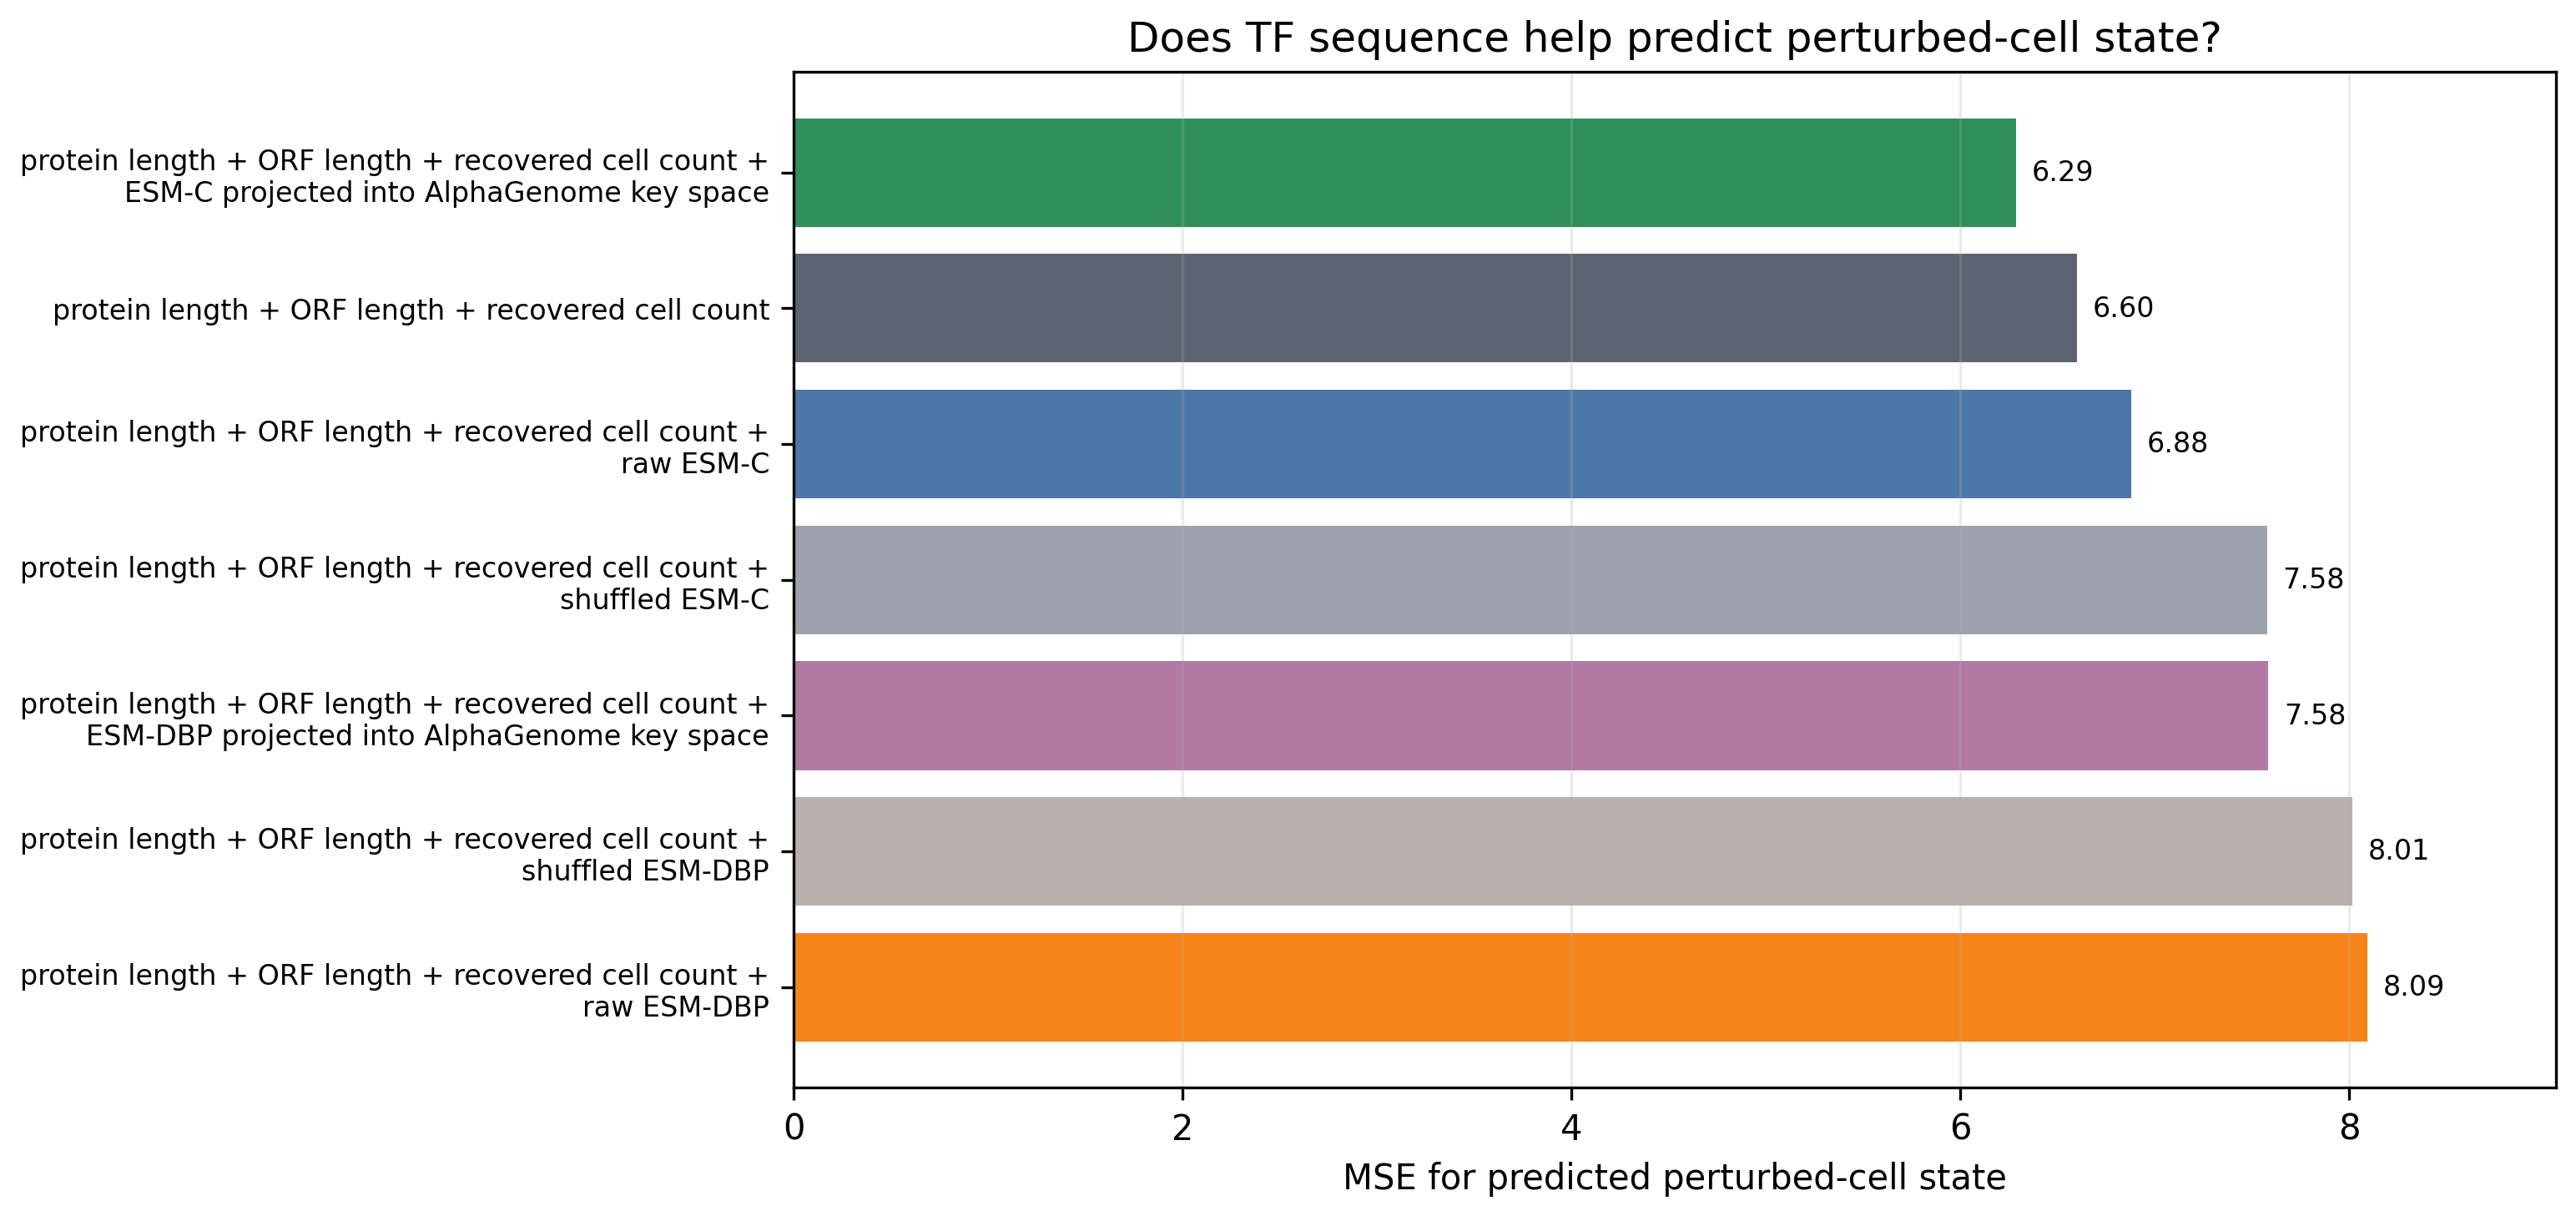
\includegraphics[width=0.68\linewidth]{figures/experiment1_controlled_overall_mse.png}
\caption{Older PCA latent MSE for predicting the perturbed cell state. This is sensitivity evidence, not the primary \scarf\ result.}
\label{fig:experiment1_controlled_overall_mse}
\end{figure}

\subsection{Encoder ablation}

\begin{table}[t]
\centering
\caption{Overall encoder ablation in the older PCA latent benchmark. Percent change is relative to using only protein length, ORF length, and recovered cell count. Negative values indicate lower MSE.}
\label{tab:ablation_results}
\resizebox{\linewidth}{!}{%
\begin{tabular}{lccc}
\toprule
\textbf{Feature set} & \textbf{MSE} & \textbf{MSE change vs three-input model} & \textbf{Interpretation} \\
\midrule
Protein length + ORF length + recovered cell count & 6.5996 & 0.0\% & Reference for this comparison \\
Protein length + ORF length + recovered cell count + \esm\ projected into \ag\ key space & 6.2879 & -4.7\% & Lowest MSE in this comparison \\
Protein length + ORF length + recovered cell count + raw \esm & 6.8774 & +4.2\% & Raw sequence embedding does not help after those three quantities \\
Raw \esm\ only & 7.3078 & +10.7\% & Weaker than measured covariates \\
Protein length + ORF length + recovered cell count + \esmdbp\ projected into \ag\ key space & 7.5832 & +14.9\% & DBP-specialized representation underperforms \esm \\
Protein length + ORF length + recovered cell count + raw \esmdbp & 8.0926 & +22.6\% & DBP-specialized raw embedding underperforms \esm \\
Protein length + ORF length + recovered cell count + shuffled \esm & 7.5761 & +14.8\% & Negative control worsens as expected \\
Protein length + ORF length + recovered cell count + shuffled \esmdbp & 8.0145 & +21.4\% & Negative control worsens as expected \\
\bottomrule
\end{tabular}%
}
\end{table}

The \scarf\ encoder diagnostic reaches the same encoder conclusion even though the main sequence feature benchmark is negative. Across all held-out genes and matched settings, positive \esmdbp-minus-\esm\ MSE differences indicate that \esm\ has lower error than \esmdbp. For example, in the all-held-out-gene setting, the median \esmdbp-minus-\esm\ MSE was \(4.10\times 10^{-9}\) after projection into \ag\ key space and \(3.47\times 10^{-9}\) for raw sequence embeddings.

\begin{figure}[t]
\centering
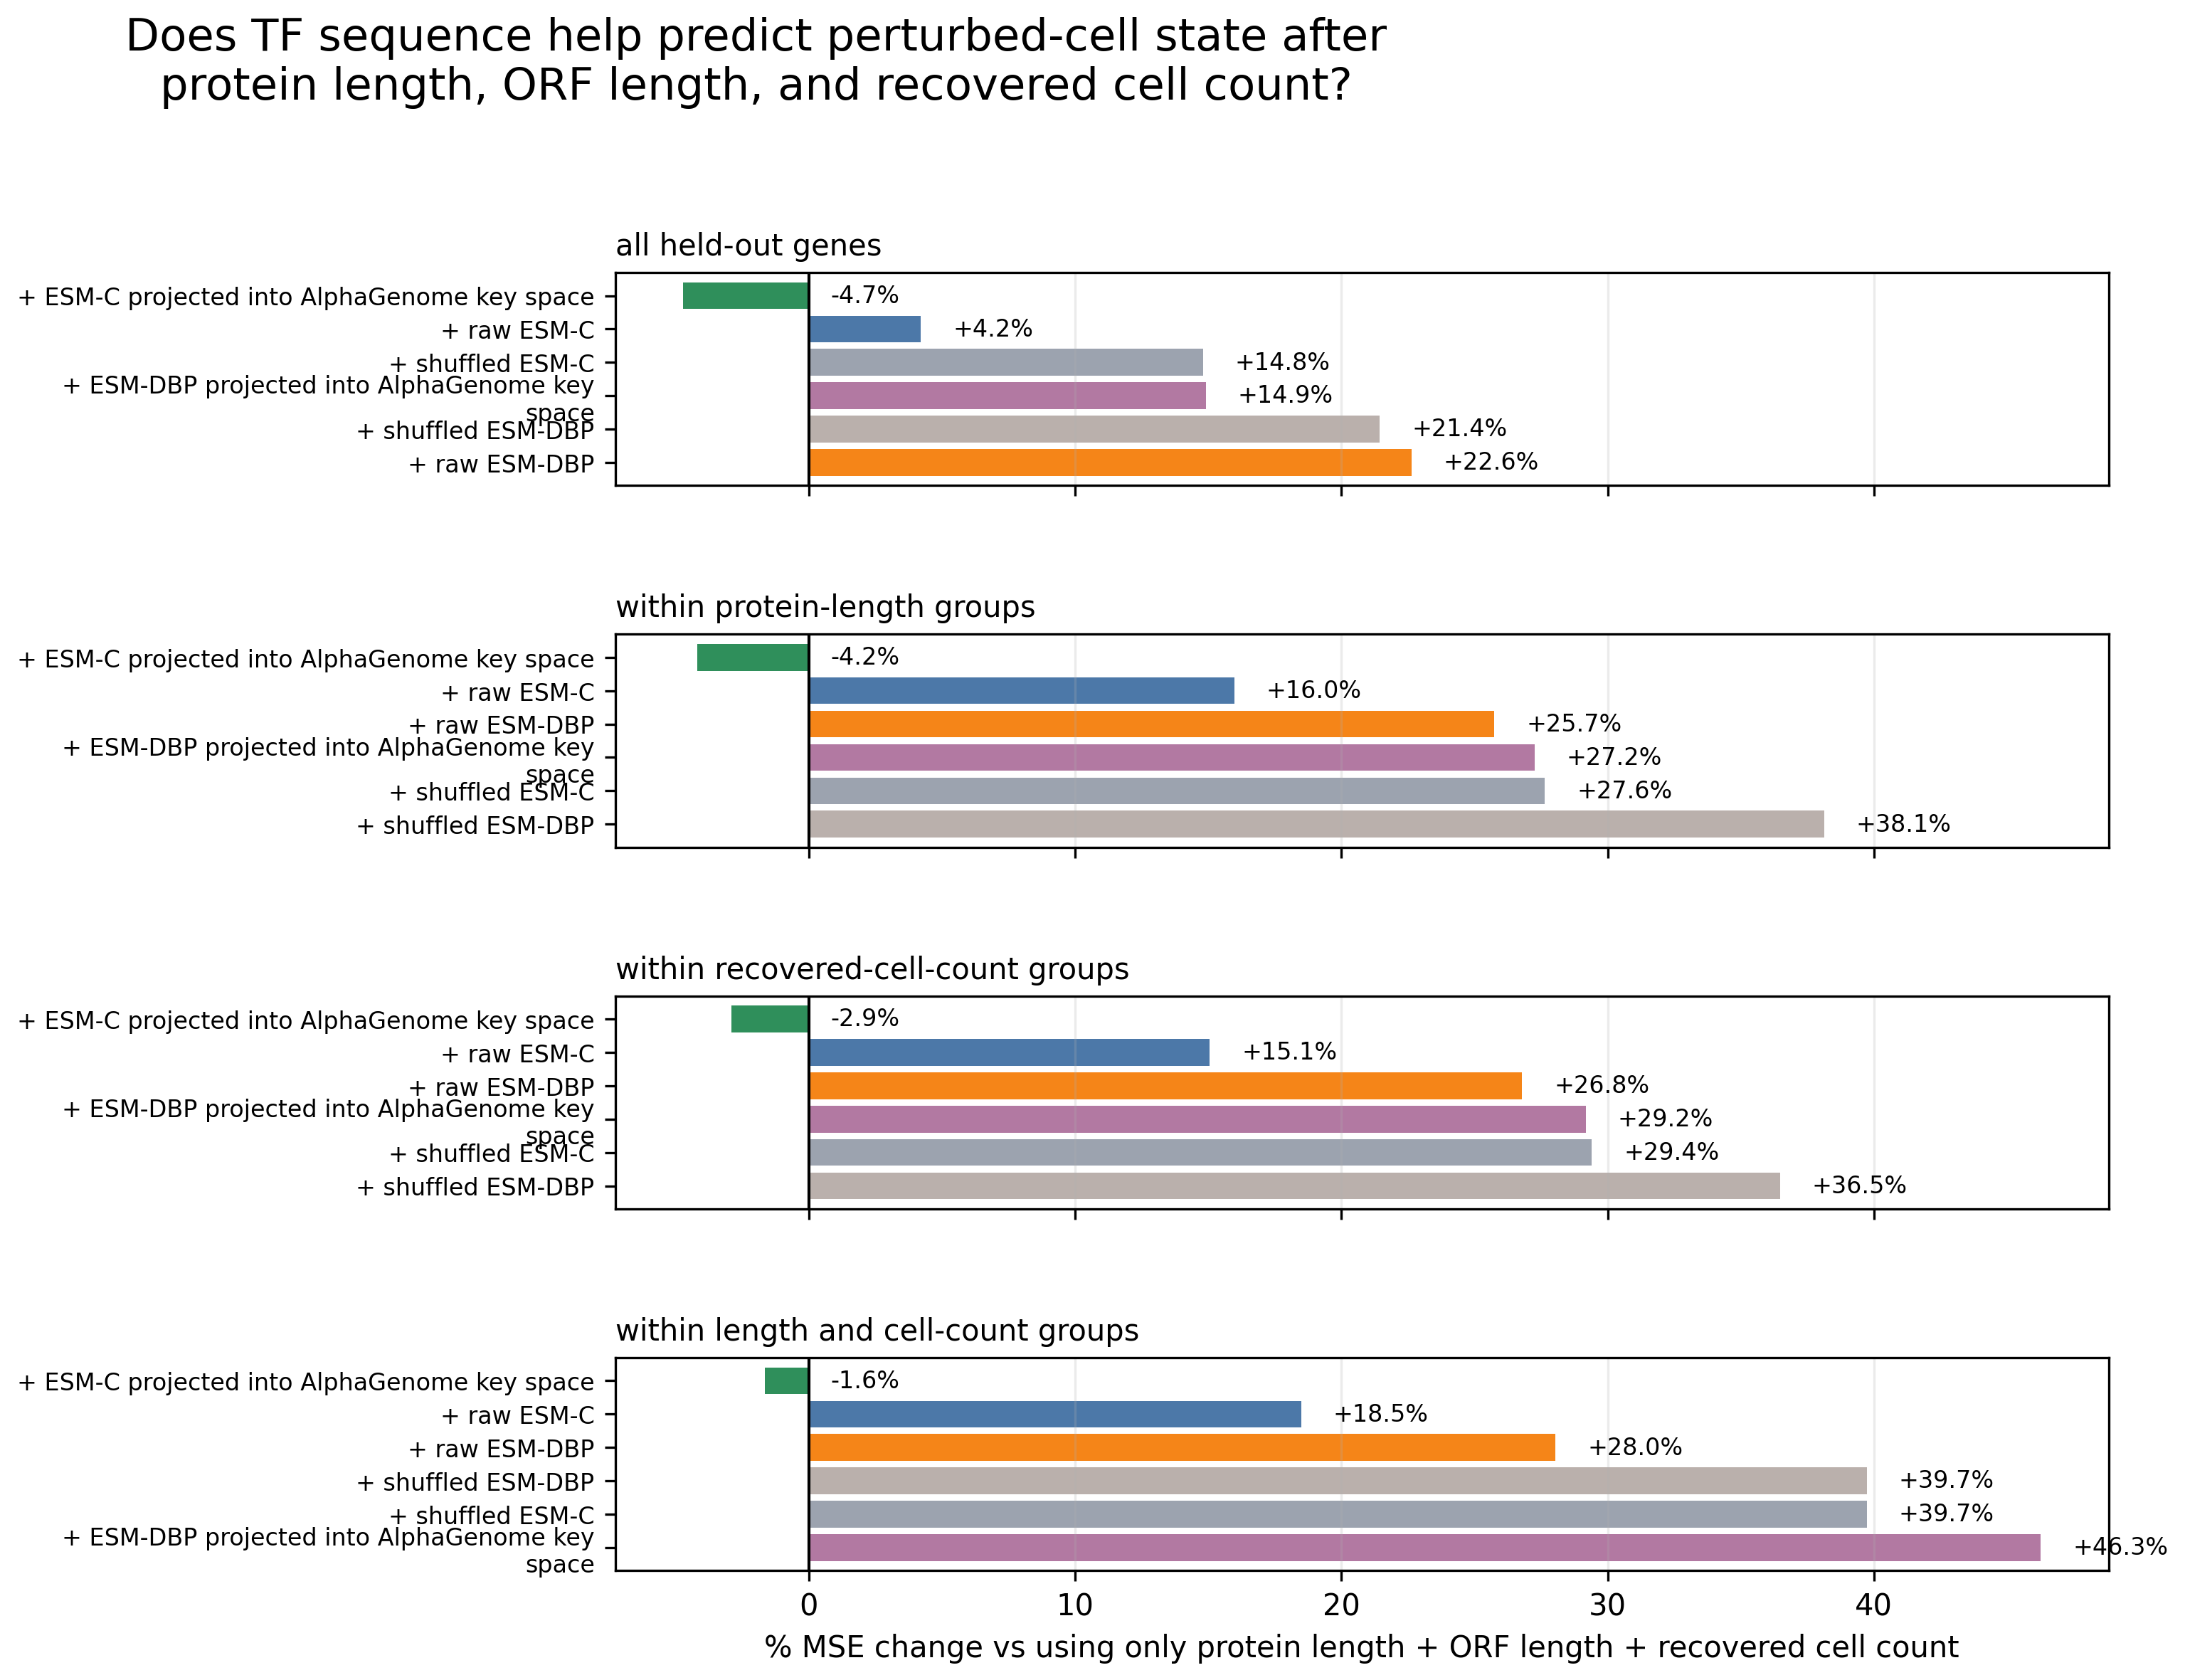
\includegraphics[width=0.68\linewidth]{figures/experiment1_sequence_after_length_cell_count.png}
\caption{Older PCA latent MSE change after adding sequence features to a model that already uses protein length, ORF length, and recovered cell count.}
\label{fig:experiment1_sequence_after_length_cell_count}
\end{figure}

\subsection{Length, ORF, and cell-count sensitivity}

\begin{table}[t]
\centering
\caption{Checks using protein length, ORF length, and recovered cell count in the older PCA-derived response representation. Lower MSE is better.}
\label{tab:length_cell_checks}
\resizebox{\linewidth}{!}{%
\begin{tabular}{lccc}
\toprule
\textbf{Control} & \textbf{MSE} & \textbf{Mean cosine similarity} & \textbf{Conclusion} \\
\midrule
Protein length only & 6.6355 & 0.4114 & Strong by itself \\
Protein length + cell count & 6.6020 & 0.3994 & Nearly matches length+cell+ORF \\
Protein length + ORF length + recovered cell count & 6.5996 & 0.3970 & Reference for sequence feature comparisons \\
Cell count only & 7.2557 & 0.3161 & Weaker alone than length-based covariates \\
\esm\ projected into \ag\ key space, protein-length groups & 6.2714 & 0.4716 & 4.2\% lower MSE \\
\esm\ projected into \ag\ key space, cell-count groups & 6.4074 & 0.3878 & 2.9\% lower MSE \\
\esm\ projected into \ag\ key space, length+cell groups & 6.4603 & 0.4604 & 1.6\% lower MSE \\
\esmdbp\ projected into \ag\ key space, length+cell groups & 9.6068 & 0.3185 & Worse \\
\bottomrule
\end{tabular}%
}
\end{table}

\section{Supplemental Retrieval and Validation Figures}
\label{app:supplemental_figures}

\begin{figure}[t]
\centering
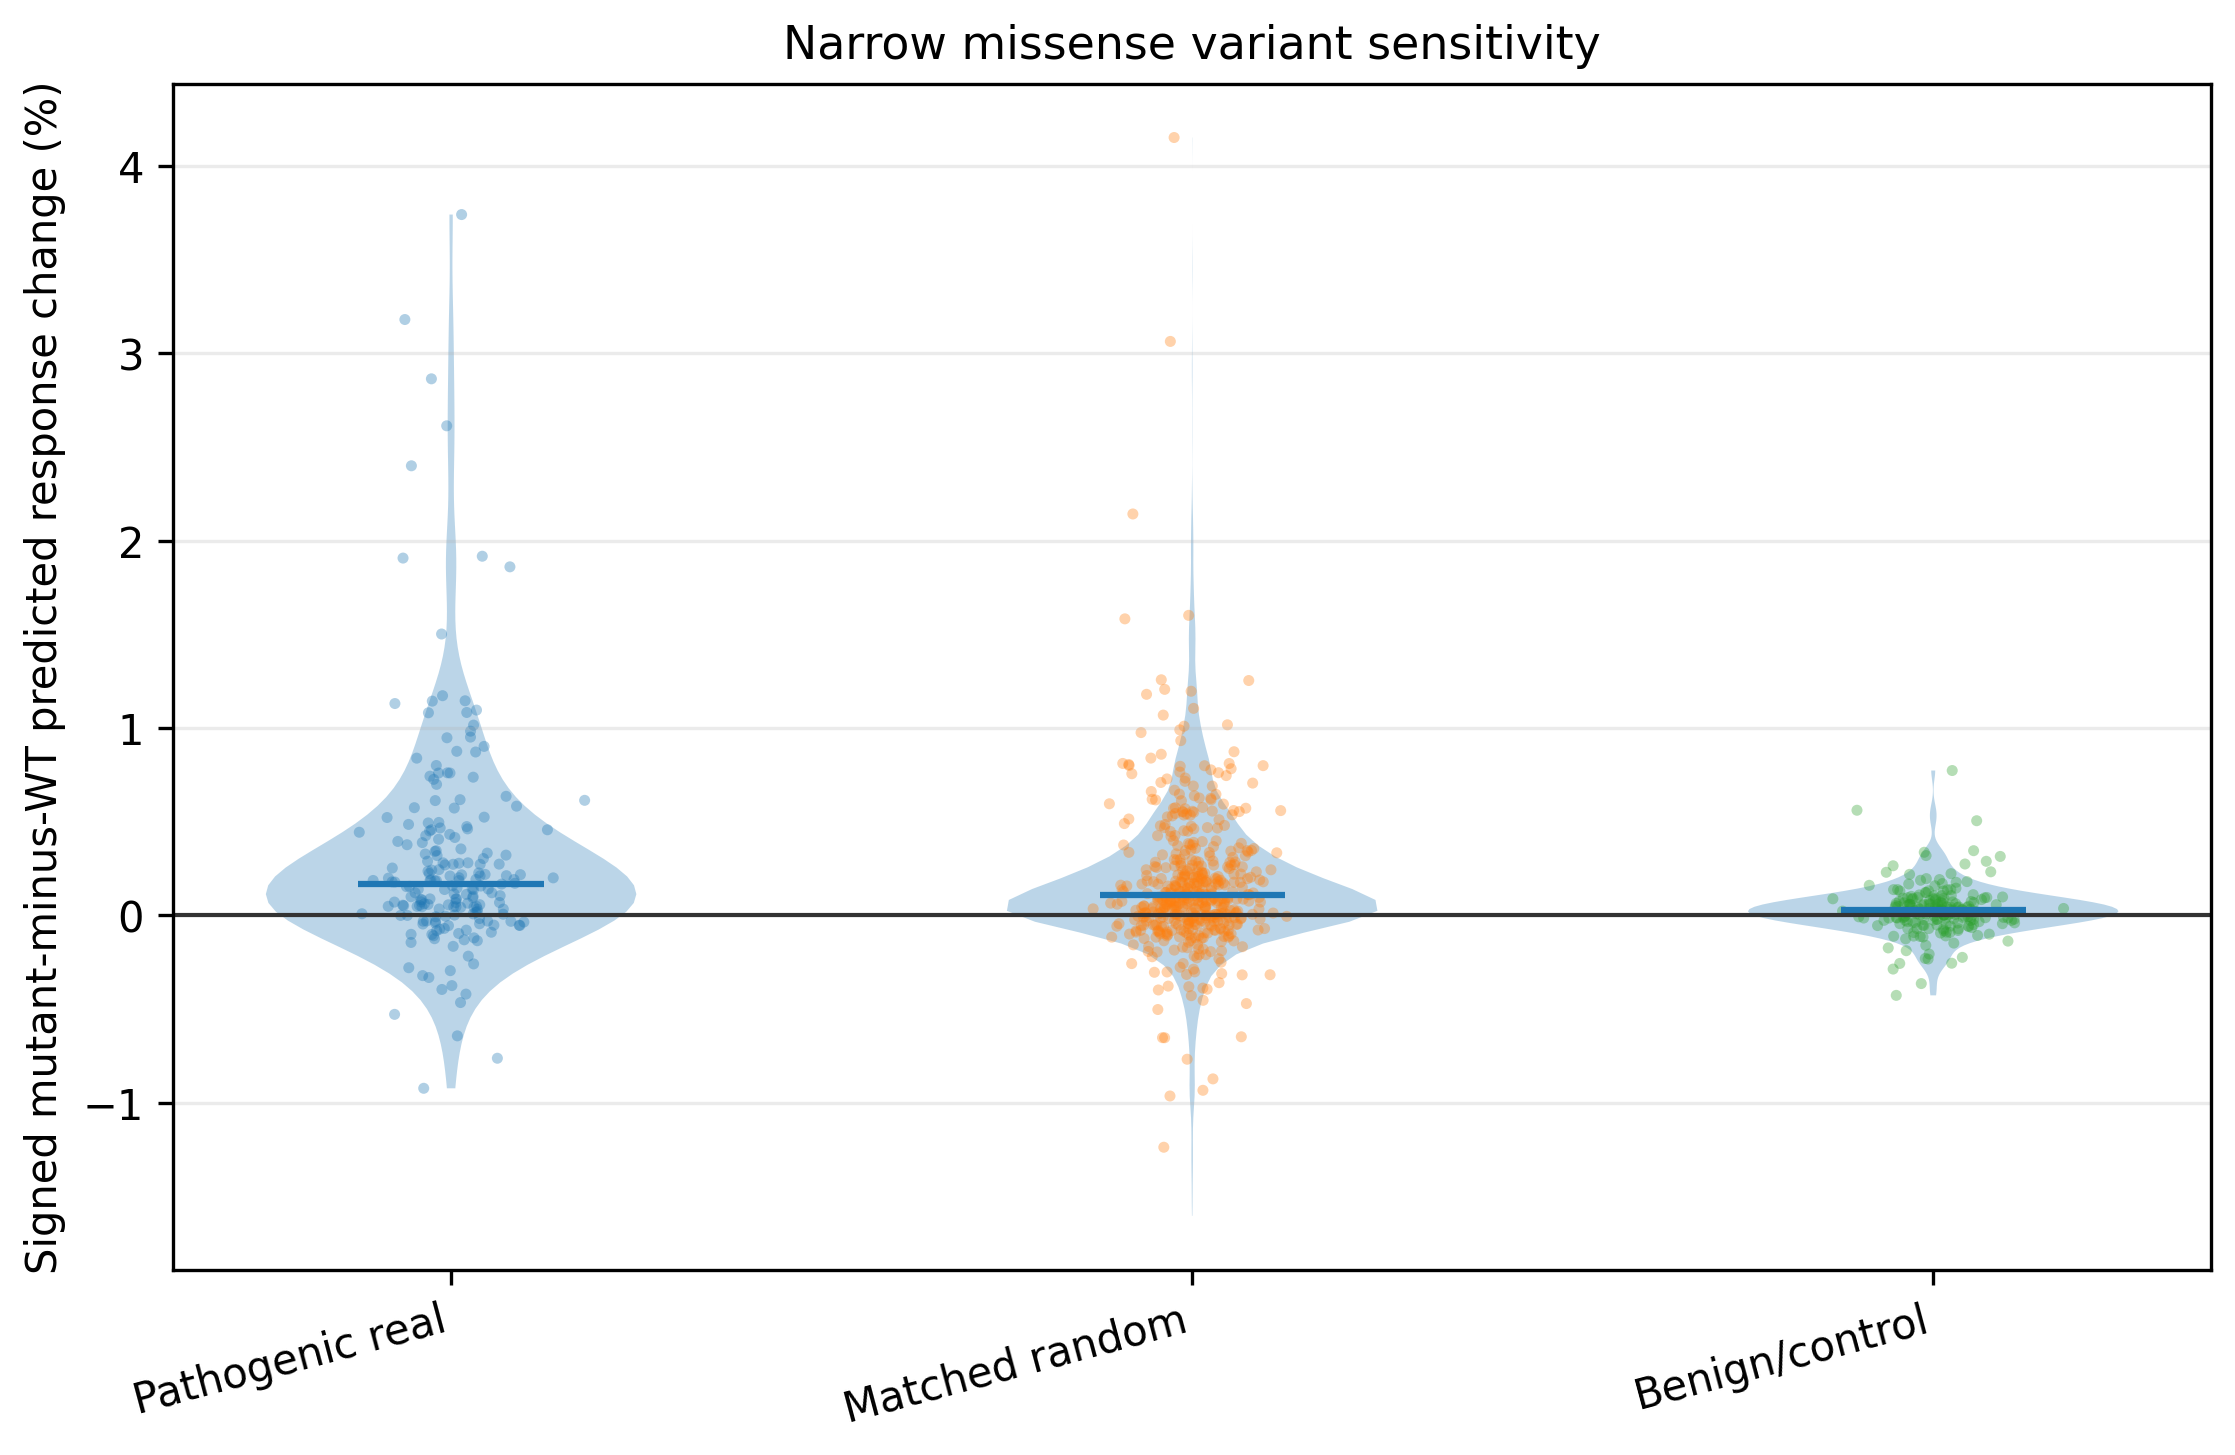
\includegraphics[width=0.68\linewidth]{figures/signed_variant_effect_violin.png}
\caption{Signed predicted perturbed cell state activity change for pathogenic variants versus matched controls. This diagnostic shows why the paper does not claim a consistent signed weakening effect.}
\label{fig:signed_variant_effect_violin}
\end{figure}

\begin{figure}[t]
\centering
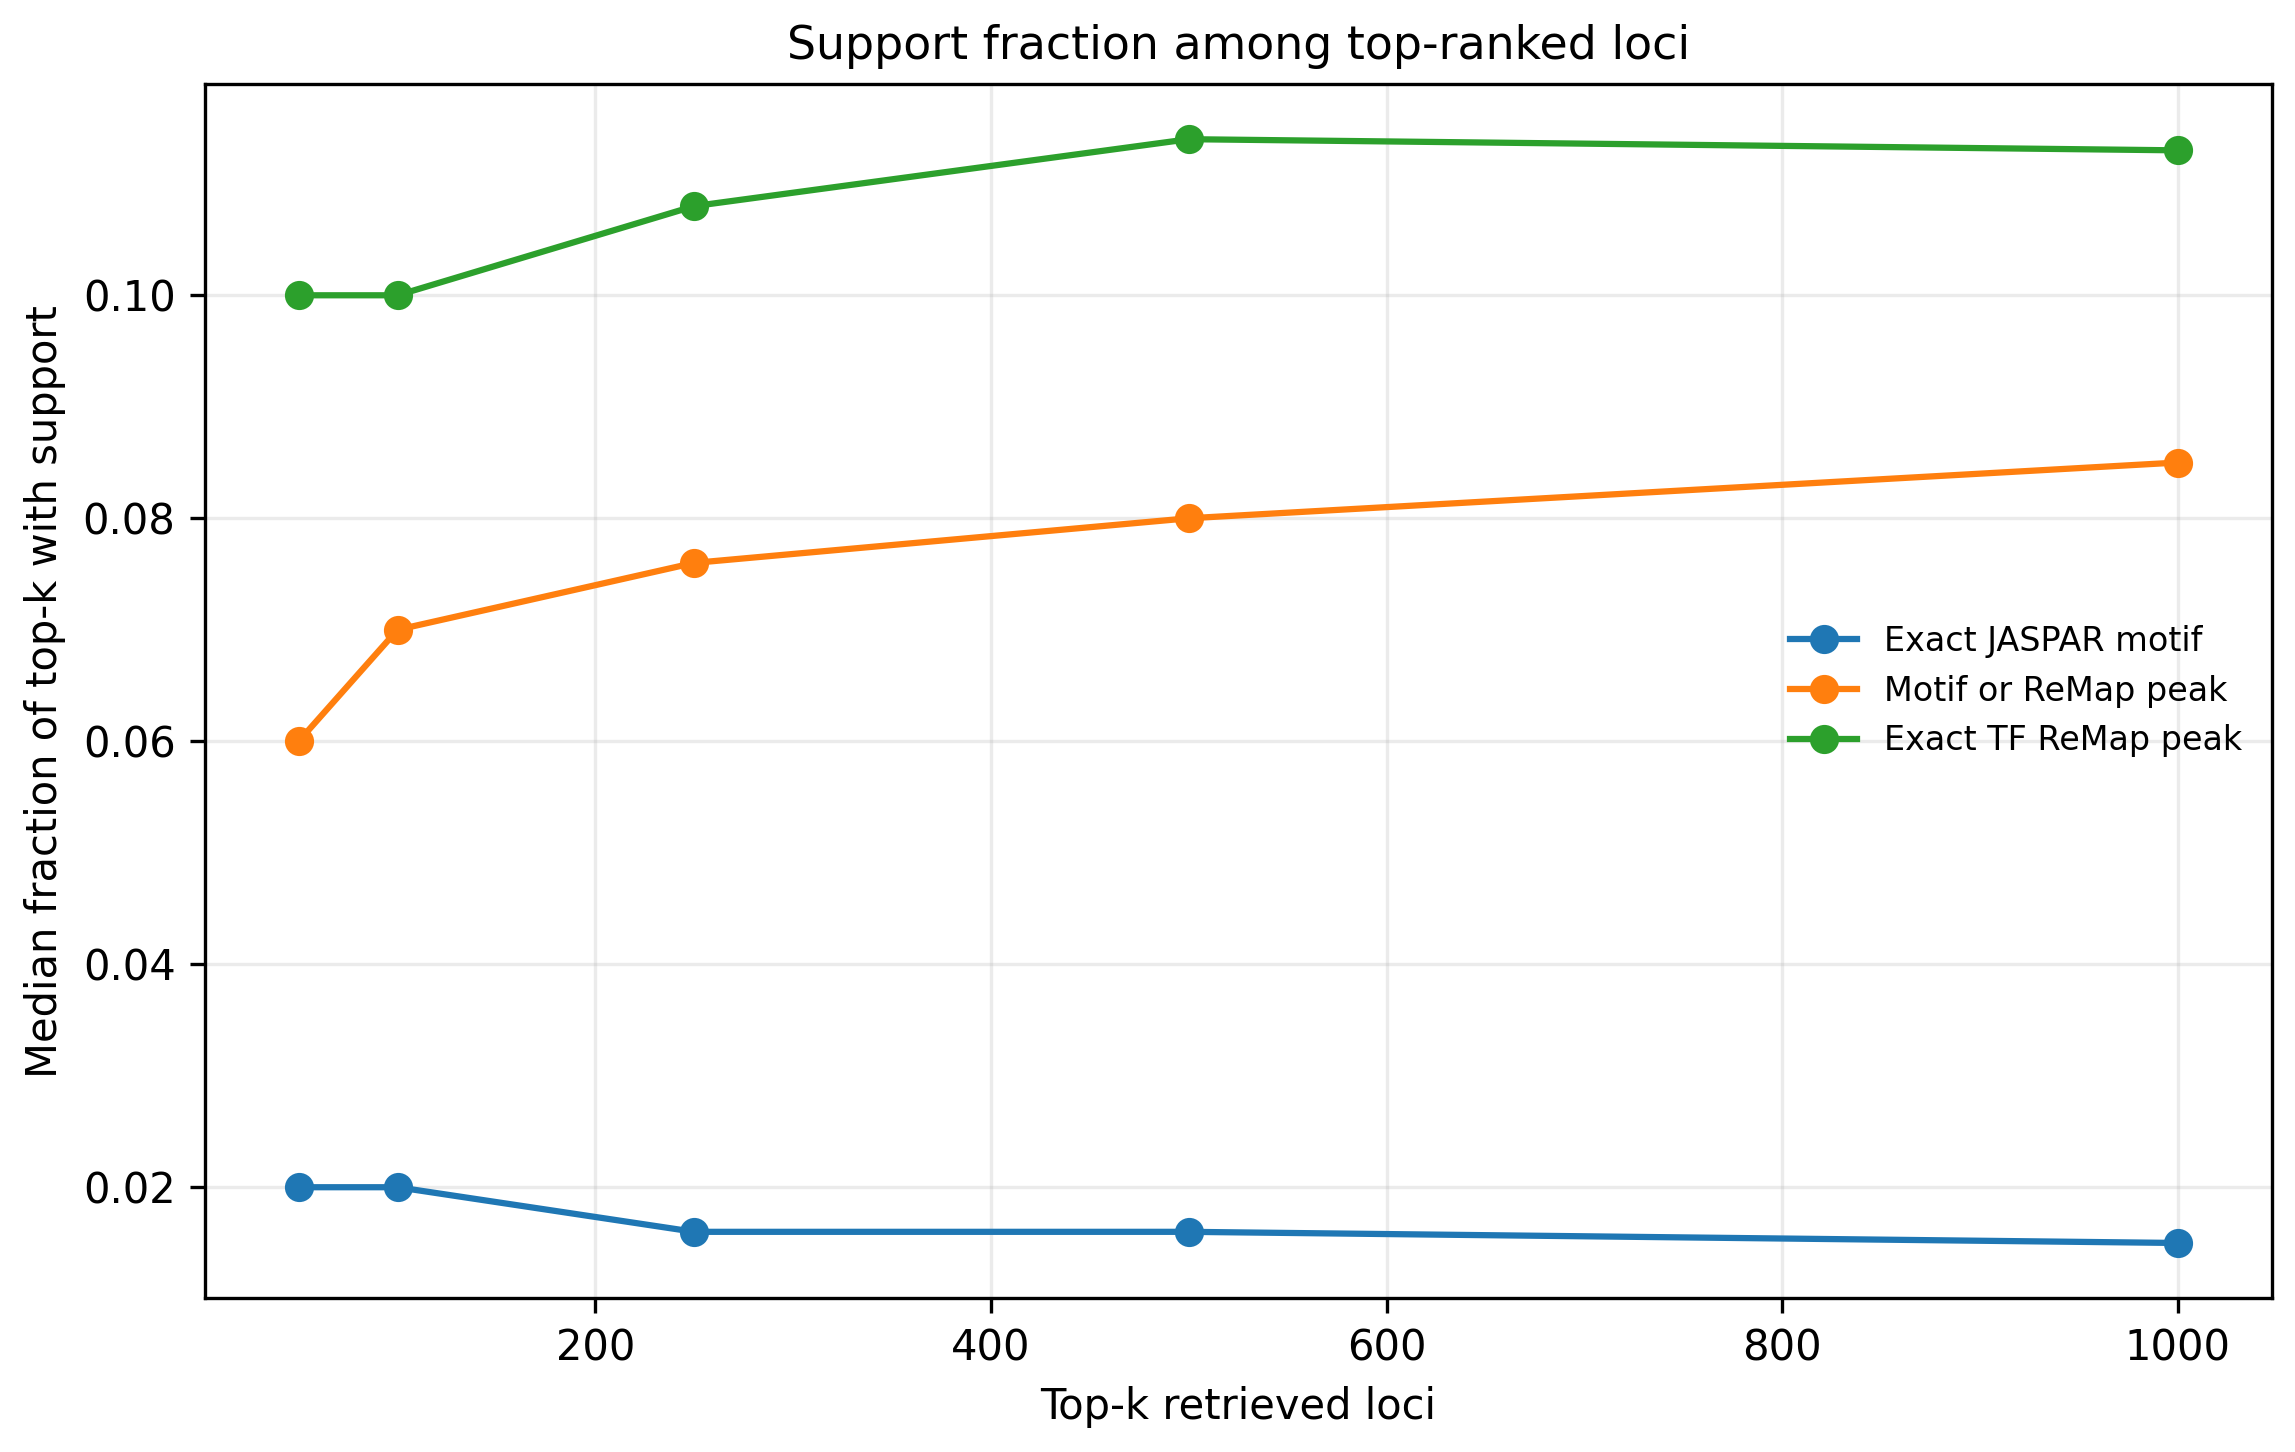
\includegraphics[width=0.68\linewidth]{figures/motif_binding_precision_by_topk.png}
\caption{Motif and ReMap support among 1~kb validation windows associated with top retrieved entries. This diagnostic asks what fraction of retrieved validation windows have exact TF symbol support; it remains modest and motivates validation that relaxes exact symbol matching where biologically justified and incorporates accessibility support.}
\label{fig:motif_binding_precision_by_topk}
\end{figure}

\section{Natural Isoform Diagnostic}
\label{app:natural_isoform}

We also tested whether natural same-gene isoform differences with interpretable domain annotations show retrieval changes that track observed response score differences. This result remains an appendix diagnostic rather than a main claim. In the conservative domain-aware analysis, 246 same-gene isoform pairs had unavailable annotations and 9 pairs had no annotated difference in domain presence. This coverage is too limited to conclude that natural isoform domain differences do not matter. The negative result mainly reflects incomplete feature mapping and coordinate annotation, not evidence that natural isoform differences fail to affect retrieval. A stronger isoform experiment would require a redesigned annotation audit across UniProt, InterPro, Pfam, Ensembl/GENCODE, and TF-specific resources before making any biological claim.

\section{Suggested Figures}
\label{app:suggested_figures}

\begin{enumerate}
    \item \textbf{Figure 1: Model overview.} TF sequence query, \ag\ locus memory, cell state bias/mask, retrieval weights, \(\mu_p\), conditional flow field.
    \item \textbf{Control panel construction.} Evidence tier counts for the benign/control variant panel, with natural evidence, tolerated substitutions supported by ortholog evidence, and legacy fallback controls separated.
    \item \textbf{Controlled perturbed cell state prediction.} Primary \scarf\ benchmark after controlling protein length, ORF length, and recovered cell count, with PCA-derived results clearly labeled as sensitivity analysis.
    \item \textbf{Variant sequence sensitivity.} Absolute disruption for pathogenic variants against matched random substitutions as the main panel; signed weakening and evidence-tiered benign/control variants as secondary panels.
    \item \textbf{Variant retrieval movement.} Chromosome-binned \ag\ key retrieval weights for WT, pathogenic mutant, and matched benign/control sequences, plus pathogenic-minus-WT signed change.
    \item \textbf{\(\beta\) sweep.} Retrieval concentration, top-\(k\) mass, and retrieval stability across \(\beta\). Include perturbed cell state performance only if a \(\beta\)-parameterized \scarf\ transport checkpoint is available.
    \item \textbf{Motif and binding support.} Precision@\(k\), recall@\(k\), rank percentile distributions, and enrichment against matched background for exact-symbol, TF-family, ReMap, and accessibility-supported windows when the family/alias maps are reliable.
    \item \textbf{Appendix figure: ESM-C vs ESM-DBP.} \scarf\ encoder diagnostic showing that \esmdbp\ does not outperform \esm\ in this setup.
    \item \textbf{Appendix figure: Length, cell count, and shuffled sequence checks.} Performance of length/cell-count inputs and shuffled sequence comparisons, labeled by response representation.
\end{enumerate}

\section{Reporting Checklist}
\label{app:reporting_checklist}

\begin{itemize}
    \item State whether \ag, \esm, and \scarf\ are frozen, adapter-tuned, or fully fine-tuned.
    \item State whether values are tied to keys.
    \item State whether retrieval is unmasked, masked by cluster, or specific to each cell.
    \item Report primary perturbed cell state metric and confidence intervals.
    \item Report retrieval entropy, top-\(k\) mass, and \(\beta\) sensitivity.
    \item Include at least one comparison that uses protein length, ORF length, and recovered cell count.
    \item Report whether conclusions persist in \scarf\ response space or remain specific to the PCA-derived response representation.
    \item Define variant labels by evidence tier; do not pool clinical benign, population tolerated, functionally neutral, and synthetic controls without showing behavior by tier.
    \item Define motif/binding-supported validation windows for \ag\ key entries, including support database, background construction, and multiple testing correction.
    \item Avoid interpreting retrieval weights as binding sites without external validation.
\end{itemize}

\end{document}
